\chapter{一般学习的可学习性}
\label{chap:convex-learning-and-stability}

前两章讨论分类：学习算法输出一个分类器，再用零一损失记录它是否预测正确。温度预测还要区分误差大小，聚类则没有给定的正确标签。这些任务都需要依据训练样本选出一个结果，再评价这个结果在新观测上的平均损失。沿用第~\ref{sec:learning-problem}节的术语，我们把完整的预测函数、聚类中心组或投影矩阵称为决策，而不把某一次预测得到的类别或数值称为学习决策。本章研究：在这些不同任务中，怎样保证算法输出的期望风险接近比较决策空间中的最低水平？

前两章给出了一条充分路线：限制假设空间的复杂程度，使同一份样本能够同时准确估计所有假设的风险，再按经验风险选择假设。二分类用VC维，多分类用零一损失类对应的图维建立这种一致收敛保证。把零一损失换成一般损失后，这条路线遇到两处改变。第一，损失取连续值，$n$个观测上的损失向量不再只有有限多种，前两章“数预测模式”的计数方法需要换成按精度衡量的容量。第二，一致收敛要求同时估计准确所有决策的风险，其中包括算法根本不会选的决策；在一般损失下，这个要求可能比学习本身更苛刻。

第二点促使我们改从算法一侧分析：不问整个决策空间有多复杂，而问算法实际输出的决策对训练样本有多敏感。具体做法是删除或替换一条训练观测，再比较两次输出在同一观测上的损失。\term{算法稳定性}（algorithmic stability）描述这种训练数据变化对输出的影响。直观地说，若某条训练观测几乎不影响输出，它对输出而言就近似一条新观测，训练损失也就能代表新数据上的损失。

稳定性只回答“训练评价是否可信”，还不能说明输出的风险是否低；算法还须在训练样本上接近最低经验风险。对具体算法同时证明这两件事，需要更多结构：凸性使优化误差可以控制，Lipschitz性把参数的移动换算成损失的变化，光滑性限制一步梯度更新怎样改变参数距离，而正则项通过强凸性直接限制解随样本的移动。本章依次建立一般学习问题、一致收敛路线和稳定性路线，最后在凸与非凸两种情形下用正则化和随机梯度下降落实这些条件。

\section{一般学习问题}
\label{sec:general-learning-problem}

为了在同一个框架中评价这些任务，沿用第~\ref{sec:learning-problem}节的设定：观测$z$属于观测空间$Z$，允许的分布组成分布族$\mathfrak P$，样本$S=(z_1,\ldots,z_n)$独立地取自某个$\mathcal P\in\mathfrak P$。损失函数$\ell(w,z)$评价决策$w$在观测$z$上的表现，损失越小表示该决策越好。算法依据样本和内部随机数$U$输出决策$A(S,U)\in\mathcal W_{\mathrm{out}}$，其中$U$表示随机初始化、随机抽样顺序等不来自数据的随机性，$\mathcal W_{\mathrm{out}}$是算法可能输出的决策全体。评价时需要一个参照：比较决策空间$\mathcal W$是我们认为“应当能做到”的那组决策，算法输出的期望风险要与$\mathcal W$中的最低期望风险比较。期望风险、经验风险和PAC保证的量词次序，分别采用定义~\ref{def:general-population-risk}--\ref{def:general-pac-learnability}。

\subsection{观测、决策与损失}

以温度预测为例，假设真实温度为20，两个模型分别预测18和10。若只记录预测是否相等，两者都被记为错误；平方损失则分别为4和100，能够反映误差大小。因此，损失函数需要根据任务中怎样评价预测来确定，而不必始终采用零一损失。

在温度预测中，观测$z$必须同时包含输入和真实温度，才能计算预测误差。一般地，$z$包含评价所需的全部信息；$w$表示被评价的选择，可以是预测函数、聚类中心或投影矩阵。损失$\ell(w,z)$越小，表示该决策在当前评价标准下越好。按定义~\ref{def:general-population-risk}与定义~\ref{def:general-empirical-risk}分别对总体和样本取平均后，学习的目标是使算法输出的期望风险接近$\inf_{w\in\mathcal W}R_{\mathcal P}(w)$。

在监督学习中，观测写为$z=(x,y)$，其中$x$是输入，$y$是用于评价的真实类别或数值。分类决策输出离散类别，回归决策输出数值；二者既可能使用不同的输出集合，也可能使用不同的损失。例如，回归的平方损失为$(w(x)-y)^2$。无论任务如何变化，经验风险都对已有样本求平均，期望风险都对新的同分布观测求平均。

没有标签的任务也可以纳入同一框架。$K$均值只观察输入$x$，决策是$K$个中心$w=(c_1,\ldots,c_K)$，损失取$x$到最近中心的平方距离$\min_j\|x-c_j\|_2^2$。例如$x=2$到中心0和5的平方距离分别为4和9，取较小值，损失为4。训练时选择使训练样本平均平方距离较小的中心；期望风险是在评价分布上计算到最近中心的期望平方距离。PCA的决策是秩为$r$的正交投影矩阵$P$，损失$\|x-Px\|_2^2$表示无法重构的部分。

统一的风险形式便于比较不同任务的学习条件，但没有消除它们在优化上的差别。$K$均值对全部中心的联合优化一般不是凸优化，不能直接使用后面的凸学习定理。此外，期望风险低只说明所选损失小，并不保证找到了唯一的“真实聚类”或“真实子空间”；许多不同的划分或子空间可以有相同的损失。应用本章定理时，仍要逐一检查具体损失和决策空间是否满足定理条件。

\subsection{可学习性的目标}

这里所说的“学会”，指达到定义~\ref{def:general-pac-learnability}中的不可知目标：算法的期望风险接近比较决策空间中的最低值，不要求最低值为零。一般任务中也不一定存在一个需要恢复的“真实标签函数”；学习目标完全由观测分布、比较决策空间和损失三者规定。除非另行说明，本章令$\mathcal W_{\mathrm{out}}=\mathcal W$，即要求输出属于比较决策空间，采用恰当输出。

学习保证针对的是一项完整设定，而不是某个模型名称。以平方损失为例，若预测值和标签都限制在有界区间内，损失也有界；放开标签的范围后，这个性质就可能消失。限制参数会改变比较决策空间，改用替代损失会改变评价目标，限制数据分布则会改变保证适用的范围。因此，修改其中任何一项，都需要核对原有风险界使用的条件是否仍成立。

零一损失自动具备的几项性质，在一般损失下都要单独假定，后面的分析也在需要时逐步增加条件。零一损失取值于$\{0,1\}$，样本平均的随机波动天然有界；一般损失可能无界，所以集中不等式需要有界性或尾部条件。零一损失下，只要能求出经验风险最小的假设，前两章就不再追问它怎样求得；对一般损失的具体算法，经验风险离最低值多远必须计算出来，这时凸性保证局部的改进方向通向全局最优。参数稍有移动，零一损失可能从0跳到1；要用“参数移动小”推出“损失变化小”，就需要Lipschitz性限制损失的变化速度。分析梯度更新时，还要知道一次更新怎样改变两条轨迹的距离，这由光滑性控制。一般学习本身并不要求损失凸或可微，这些条件只服务于具体推导，不能当成所有学习问题的共同前提。

\section{一致收敛}
\label{sec:real-valued-classes}

把零一损失换成一般损失后，每个决策的期望风险仍要由样本来估计。但损失取值不再只有0和1，为利用前面的理论，先把每个决策对应一个损失函数：所有决策对应的损失函数组成损失类
\[
 \mathcal F_\ell=\{z\mapsto\ell(w,z):w\in\mathcal W\},
\]
风险是损失对总体的平均，所以要控制的是这组函数的样本平均与总体平均之差。这里必须使用损失类，而不能直接使用预测函数类：同一组预测函数配上不同损失，得到的函数类可能在有界性和复杂度上完全不同；预测函数本身的维度，不能不经转换就代入风险界。

% 保留旧位置锚点；在一般损失上使用一致收敛条件。
\phantomsection\label{def:general-uniform-convergence}
与第~\ref{sec:binary-uniform-convergence}节相同，仍要求同一份样本把整个损失类中每个函数的期望都估计准确。对任意$\eta,\delta\in(0,1)$，若存在一个充分样本量$n_{\mathrm{uc}}(\eta,\delta)$，使每个允许分布$\mathcal P$和每个$n\geq n_{\mathrm{uc}}(\eta,\delta)$都满足
\[
 \mathbb P_{S\sim\mathcal P^n}\!\left\{
 \sup_{w\in\mathcal W}|\hat R_S(w)-R_{\mathcal P}(w)|\leq\eta
 \right\}\geq1-\delta.
\]
这就是一般损失类上的一致收敛要求（集中不等式与依概率收敛的一般概念可参考\BookVolumeRef{vol:mathematical-preliminaries-lower}{卷2《数学准备：概率、因果与决策》}）。
上确界不超过$\eta$，要求同一份样本对所有决策的风险估计都达到精度$\eta$。样本量可以随决策空间、损失、精度和置信度改变，但对允许族中的每个分布必须相同，这称为在该族上统一的保证。只有当允许族包含观测空间上的全部相关分布时，才进一步称为分布无关保证。以下各类稳定性也保留同一区分：先要求速率在指定的允许族上统一，取全分布族时再称分布无关。

怎样判断一个损失类能否满足这一要求？零一损失下，$n$个观测上的损失向量属于$\{0,1\}^n$，至多$2^n$种，VC维限制了实际出现的种数，计数论证由此展开。换成平方损失后，即使只有一个观测$z=(x,y)$，预测值连续变化也会给出连续多种损失值，计数不再有意义。我们需要一种只区分“差异足够大”的函数的容量，下一小节把前章的打散概念扩展为函数值与阈值的比较。

\subsection{伪维与胖打散维}

VC维检验的是：函数类能否在$m$个输入上实现全部$2^m$种0/1标注。实值函数没有现成的0/1标注，但可以人为制造：在$m$个不同输入$x_1,\ldots,x_m$处各指定一个阈值$r_1,\ldots,r_m$，记录函数值位于阈值的上方还是下方。若对每种高低模式$b\in\{0,1\}^m$，都有$f\in\mathcal F$使$b_j=1$时$f(x_j)\geq r_j$、$b_j=0$时$f(x_j)<r_j$，就说这些输入被伪打散。\term{伪维}（pseudo-dimension）是能够这样打散的输入个数的上确界；它衡量的仍是“能实现多少种高低组合”，不是损失值的个数。

伪打散允许函数值只比阈值高出一点点。可是风险估计只要求精度$\eta$，相差远小于$\eta$的两个函数无须区分。\term{胖打散维}（fat-shattering dimension）$\operatorname{fat}_\gamma(\mathcal F)$因此加上间隔：高于阈值时至少高出$\gamma$，低于阈值时至少低出$\gamma$，即$f(x_j)\geq r_j+\gamma$或$f(x_j)\leq r_j-\gamma$。尺度$\gamma$越小，要求越宽松，$\operatorname{fat}_\gamma$随$\gamma$减小而不减（相关组合定义可参考\BookVolumeRef{vol:mathematical-preliminaries-upper}{卷1《数学准备：计算、分析与几何》}）。对二值函数取阈值$1/2$即回到VC打散，所以二值函数的伪维等于VC维；多分类标签若只是名称，则不能通过任意编号引入大小关系，再用伪维代替多分类维度。

阈值比较与带间隔比较的差别，可以用一个函数值随位置衰减的例子说明。令$X=\mathbb N$，每个有限集$C\subset\mathbb N$对应一个函数：$i\in C$时$f_C(i)=1/i$，$i\notin C$时$f_C(i)=0$。任取有限多个点$i_1,\ldots,i_m$，在每个点$i_j$处把阈值设为$r_j=1/(2i_j)$，再通过选择$C$决定该点函数值在阈值上方（取$1/i_j$）还是下方（取0），就能实现全部$2^m$种高低模式，所以伪维无限。胖打散则要求每个点的两个可选值至少相差$2\gamma$，而这里的差只能是$1/i_j$，所以被胖打散的点必须满足$i_j\leq1/(2\gamma)$，这样的点只有有限个，每个正尺度$\gamma$下的胖打散维都有限。下一小节回答：这两种区分能力中，哪一种能控制风险估计的统一偏差。

\subsection{一致收敛与期望风险}

风险估计只要求达到指定精度$\eta$，相应的容量也应在这个数值尺度上衡量：函数之间在每个点上的差异小于精度时，没有必要区分。下面的定理表明，对取值于$[0,1]$的函数类，在允许所有概率分布时，一致收敛成立，当且仅当每个正尺度的胖打散维都有限。取值于一般有界区间的函数，可以先平移缩放到$[0,1]$。若分布族$\mathfrak P$较小，有限胖打散维仍足以保证一致收敛，但反方向可能不成立：受限分布未必能让函数之间的全部差异表现出来。无界损失还需要额外的尾部控制。以下涉及上确界、算法和期望的地方，都假定满足所需的可测性条件。

\begin{theorem}[胖打散维与一致收敛]
\label{thm:fat-uniform-convergence}
设$(X,\mathcal A)$为可测空间，$\mathcal F$为非空的$[0,1]$值可测函数空间。
假定存在可数子空间$\mathcal F_0\subseteq\mathcal F$，使每个$f\in\mathcal F$都是
$\mathcal F_0$中某个函数序列的逐点极限。则以下两个命题等价：
\begin{enumerate}
 \item 对每个$\gamma>0$，$\operatorname{fat}_{\gamma}(\mathcal F)<\infty$。
 \item 对任意$\eta,\delta\in(0,1)$，存在整数$n_0=n_0(\mathcal F,\eta,\delta)$，
 使任意$X$上的概率分布$\mathcal P$和任意$n\geq n_0$均满足
 \[
 \mathbb P_{(x_1,\ldots,x_n)\sim\mathcal P^n}\!\left\{
 \sup_{f\in\mathcal F}
 \left|\frac1n\sum_{i=1}^n f(x_i)-\mathbb E_{x\sim\mathcal P}f(x)\right|
 >\eta\right\}\leq\delta.
 \]
\end{enumerate}
\end{theorem}

定理两边的量词要分别看清。维度条件要求对每个$\gamma>0$，该尺度下的胖打散维都有限，但不同$\gamma$对应的维度可以随$\gamma$减小而增大。收敛条件要求同一个$n_0$适用于所有分布。可数子空间$\mathcal F_0$用来处理上确界的可测性；$\mathcal F$本身可数时直接取$\mathcal F_0=\mathcal F$。有界性还保证逐点逼近的函数在期望上也逼近，因此可以用可数子空间控制概率事件。要把定理用于学习问题，只需把$X$换成观测空间$Z$、令$\mathcal F=\mathcal F_\ell$，并核对有界性和可测性条件。

这一等价刻画的经典形式见学习理论教材\scite{shalevshwartz2014}，更精细的一致收敛上界见\scite{colomboni2023fat}。充分性证明仍采用副样本的想法：用另一份独立样本代替总体，把问题化为有限个点上的比较。困难在于实值函数无法靠精确计数函数值向量处理，有限输入上不同的损失向量有无穷多个。做法是把彼此相差不足某个精度（例如$\eta/4$）的损失向量归为一组，每组用一个代表向量近似。这样一组代表称为覆盖，所需代表的最少个数称为覆盖数。胖打散维与覆盖数的关系，类似VC维与增长函数的关系：适当尺度的胖打散维有限时，覆盖数的对数至多与该维度乘以样本量对数的平方同阶，远小于样本量本身。对有限个代表向量应用集中不等式并取并集界，再加上近似带来的误差，就得到全部函数的偏差控制。必要性则从某个正尺度上任意大的打散点集出发：打散点远多于样本量时，在这些点上取均匀分布，任意一份样本都只覆盖其中一小部分；由于打散允许在抽到与未抽到的点上分别取阈值两侧、相差至少$2\gamma$的值，总能找到经验平均与总体平均相差约$\gamma$量级的函数，统一偏差因而不趋于零。完整证明还需要覆盖数的组合估计，这里只说明证明路径。

胖打散比伪打散要求更强，所以有限伪维是一致收敛的充分条件；上面的衰减例子说明它不是必要条件。若希望直接利用当前样本估计复杂度，也可以把第~\ref{chap:binary-learnability}章的Rademacher复杂度用于一般损失类，再据此控制期望风险。

一致收敛只说明样本能把每个决策的风险估计到精度$\eta$，还没有说明算法选出的决策好不好。下面的定理把它与选择规则接起来。算法不必精确求出经验最优，只要求经验风险比最低值至多高出$\alpha$，这为数值优化留出余地。结论中的$2\eta$来自两次换算：一次把输出的期望风险换成经验风险，一次把比较决策的经验风险换回期望风险，每次至多差$\eta$。

\begin{theorem}[一致收敛推出一般学习保证]
\label{thm:general-uniform-pac}
设$(Z,\mathcal Z)$为可测观测空间，
$(\mathcal W,\mathcal B_{\mathcal W})$为非空可测决策空间，
$\mathfrak P$为$Z$上的一族概率分布。设
$\ell:\mathcal W\times Z\to\mathbb R$可测，且对每个
$\mathcal P\in\mathfrak P$和$w\in\mathcal W$都有
$\ell(w,\cdot)\in L^1(\mathcal P)$。对$S=(z_1,\ldots,z_n)\sim\mathcal P^n$定义
\[
 R_{\mathcal P}(w)=\mathbb E_{z\sim\mathcal P}\ell(w,z),
 \qquad
 \hat R_S(w)=\frac1n\sum_{i=1}^n\ell(w,z_i),
\]
并假定以下上确界及相关事件可测。令确定性算法
$A_n:Z^n\to\mathcal W$可测，并在固定$n$时简记$A=A_n$。若某份样本$S$及算法输出满足
\[
 \sup_w|\hat R_S(w)-R_{\mathcal P}(w)|\leq\eta,\qquad
 \hat R_S(A_n(S))\leq\inf_w\hat R_S(w)+\alpha,
\]
其中$\eta,\alpha\geq0$，则
\[
 R_{\mathcal P}(A_n(S))\leq\inf_w R_{\mathcal P}(w)+2\eta+\alpha.
\]
若对任意$\eta,\delta\in(0,1)$，存在不依赖$\mathcal P$的整数
$n_{\mathrm{uc}}(\eta,\delta)$，使所有$n\geq n_{\mathrm{uc}}(\eta,\delta)$均满足
\[
 \mathbb P_{S\sim\mathcal P^n}\!\left\{
 \sup_{w\in\mathcal W}|\hat R_S(w)-R_{\mathcal P}(w)|\leq\eta
 \right\}\geq1-\delta
 \quad\text{对每个 }\mathcal P\in\mathfrak P,
\]
且存在不依赖$\mathcal P$的$\alpha_n\to0$，使每份$S\in Z^n$都满足
\[
 \hat R_S(A_n(S))\leq\inf_{w\in\mathcal W}\hat R_S(w)+\alpha_n,
\]
则该算法相对于允许族$\mathfrak P$统一地PAC学习此问题；只有$\mathfrak P$包含全部相关分布时，才称为分布无关PAC学习。
\end{theorem}
\begin{proof}
对任意固定比较决策$w$，依次比较期望风险、经验风险和经验最优值，得到
\begin{align*}
 R_{\mathcal P}(A(S))&\leq\hat R_S(A(S))+\eta\\
 &\leq\hat R_S(w)+\alpha+\eta\\
 &\leq R_{\mathcal P}(w)+\alpha+2\eta.
\end{align*}
对$w$取下确界即可。取$\eta\leq\varepsilon/4$、$\alpha\leq\varepsilon/2$，
并让一致收敛事件的概率至少为$1-\delta$，便得到PAC保证。
\end{proof}

上述证明只在期望风险、经验风险和经验最优值之间比较，没有用到凸性。它说明一致收敛配合足够小的经验优化误差就能保证学习。还需检验反方向：一个问题可学习，是否必须要求同一份样本把所有决策的风险都估计准确？下一小节给出否定的例子。

\subsection{一致收敛不是必要条件}

检验反方向时，可以构造一个决策空间：其中有一个已知的好决策，另有许多决策会使经验评价严重失真。取$Z=\mathbb N$，$w_0$是一个特殊决策，每个有限集$C\subset\mathbb N$也是一个决策，损失定义为
\[
 \ell(w_0,z)=0,\qquad \ell(C,z)=\mathbb I\{z\notin C\}.
\]
$w_0$在任何观测上都没有损失；集合决策$C$只在观测不属于$C$时受罚。所有有限子集是可数的，因此这个损失类满足本部分要求的可数逼近条件。

\begin{theorem}[可学习性不推出一致收敛]
\label{thm:general-learning-without-uniform}
令可测观测空间为$(Z,2^Z)$，其中$Z=\mathbb N$；令可测决策空间为
$\mathcal W=\{w_0\}\cup\{C:C\subset\mathbb N,\ C\text{有限}\}$及其幂集，
并允许$Z$上的所有概率分布。定义可测且取值于$\{0,1\}$的损失
\[
 \ell(w_0,z)=0,\qquad
 \ell(C,z)=\mathbb I\{z\notin C\}.
\]
对每个$n\geq1$、每个$Z$上的概率分布$\mathcal P$及
$S\sim\mathcal P^n$，确定性算法$A_n:Z^n\to\mathcal W$定义为$A_n(S)=w_0$。
该损失有界，因而算法的训练损失与独立测试损失均可积。
则$(A_n)_{n\geq1}$分布无关PAC学习该问题，但损失函数空间
$\{z\mapsto\ell(w,z):w\in\mathcal W\}$不满足分布无关的一致收敛。
\end{theorem}
\begin{proof}
始终输出$w_0$的算法在每个分布下都具有零期望风险，因此达到最优。
另一方面，对每个样本量$n$，令$\mathcal P_n$为
$\{1,\ldots,2n\}$上的均匀分布。对任何$S\sim\mathcal P_n^n$，
记其出现过的观测构成的集合为$C_S$。由于$|C_S|\leq n$，有
\[
 \hat R_S(C_S)=0,\qquad R_{\mathcal P_n}(C_S)\geq\frac12.
\]
前者因为每个样本点都属于$C_S$，后者因为$C_S$至多覆盖$\mathcal P_n$支持集的一半。
一致收敛要求同一个样本量适用于所有分布，但每个$n$都有上述$\mathcal P_n$使统一偏差
以概率1至少为$1/2$，所以分布无关的一致收敛不成立。
\end{proof}

在这个决策空间中，始终输出$w_0$和输出样本中出现过的观测组成的集合$C_S$，经验风险都是0，因而都是ERM。但在证明使用的分布$\mathcal P_n$下，前者的期望风险为0，后者至少为$1/2$。经验最优只规定选择经验风险最小的决策，没有规定在多个并列最优者中如何选择；而这里的选择方式足以决定学习成败。一个成功的算法可以保留整个决策空间，始终输出$w_0$，并不需要删去那些风险估计失真的集合决策。

这个构造并不否定二分类基本定理，因为二分类损失的结构不允许出现$w_0$这样的决策。二分类的观测也是$z=(x,y)$，但损失由预测类别与标签是否相等决定：对同一个输入$x$，同一个分类器在$(x,0)$和$(x,1)$上不可能都取得零损失。这里的$w_0$却对全部观测零损失，一般损失允许这样的特殊决策，所以一致收敛不成立时仍可学习。下一节转而直接分析算法的选择过程，寻找控制泛化的另一条途径。

\section{算法稳定性与可学习性}
\label{sec:algorithmic-stability}

上一节的两个ERM面对同一个决策空间，只因为在并列最优者之间的选择方式不同，期望风险就完全不同。因此本节固定算法本身，考察训练样本改变时它的输出如何变化。

为什么训练样本的微小改变与泛化有关？训练损失偏乐观，是因为算法用这些观测挑选了输出，输出可能恰好迁就了它们。设想把第$i$条观测换成一条新观测重新训练：若输出几乎不变，那么原输出在$z_i$上的损失，就接近一个从未见过$z_i$的输出在$z_i$上的损失，而后者正是对新数据的无偏评价。于是“替换一条观测，输出损失变化很小”可以转化为“训练损失接近期望风险”。这一推理只涉及算法实际产生的输出，不需要估计决策空间中其他决策的风险，正好避开了上一节一致收敛过强的问题。

按这一思路构造的条件有三个可调整之处：直接比较损失，还是先比较参数距离；删除一条观测（样本量变为$n-1$）还是替换一条（样本量不变）；要求每对样本都受控，还是按样本出现的概率取平均。这几项可以组合，例如参数距离也可以按平均方式控制，所以下文各小节的名称不是互斥类别。信息方法则不逐次比较两份训练结果，而衡量输出与训练样本整体的统计依赖。各种条件最终都服务于同一个量的估计，下面先把这个量写出来。

在把稳定性与学习联系起来之前，先区分两个需要控制的量。\term{期望泛化差}比较算法在独立新观测和训练观测上的平均表现：
\[
 \mathbb E_S[R_{\mathcal P}(A(S))-\hat R_S(A(S))].
\]
它是一个有符号的量：为正时，表示经验风险平均而言低估了期望风险。\term{超额期望风险}则比较输出的期望风险与比较决策空间中的风险下确界：
\[
 R_{\mathcal P}(A(S))-\inf_{w\in\mathcal W}R_{\mathcal P}(w).
\]
期望泛化差的绝对值小，只说明重复抽样、训练后的两种平均风险接近；不同运行的正负偏差仍可能相互抵消。即使这两个平均风险完全相等，它们也可能同时很大：在$[0,1]$上用平方损失，若观测恒为1而算法始终输出0，训练风险与期望风险都是1，泛化差为零，而输出1的风险为零。超额期望风险则以比较决策空间的风险下确界为基准，反映输出离最优风险还有多远。为从前者得到后者，我们还需要算法在训练样本上接近经验最优，即输出的经验风险减去$\inf_{w\in\mathcal W}\hat R_S(w)$所得的\term{经验优化误差}（empirical optimization error）要小；上例中这一误差恒为1。下一个定理把这两项要求合并起来，不要求风险下确界由某个决策取到。

\begin{theorem}[期望泛化差与经验最优性]
\label{thm:generalization-optimization-learning}
设$(Z,\mathcal Z)$与$(\mathcal W,\mathcal B_{\mathcal W})$分别为可测观测空间和
非空可测决策空间，$\ell:\mathcal W\times Z\to\mathbb R$可测。
对每个允许分布$\mathcal P$，令$S=(z_1,\ldots,z_n)\sim\mathcal P^n$，
令算法内部随机数$U$独立于$S$，并令可测算法
$A_n:Z^n\times\mathcal U\to\mathcal W$输出$A_n(S,U)$，并在固定$n$时简记
$A=A_n$。再令
$z\sim\mathcal P$独立于$S,U$，定义
\[
 R_{\mathcal P}(w)=\mathbb E_{z\sim\mathcal P}\ell(w,z),
 \qquad
 \hat R_S(w)=\frac1n\sum_{i=1}^n\ell(w,z_i).
\]
假定$\ell(A_n(S,U),z)$及每个$\ell(A_n(S,U),z_i)$均可积；
$\inf_{w\in\mathcal W}R_{\mathcal P}(w)$为有限实数，且
$\inf_{w\in\mathcal W}\hat R_S(w)$可测且几乎处处为有限实数。若对所有允许分布均有
\[
 \mathbb E_{S,U}[R_{\mathcal P}(A_n(S,U))-\hat R_S(A_n(S,U))]\leq g_n,
\]
以及
\[
 \mathbb E_{S,U}\!\left[\hat R_S(A_n(S,U))-
 \inf_{w\in\mathcal W}\hat R_S(w)\right]\leq\rho_n,
\]
其中$g_n,\rho_n$为不依赖具体分布的非负数，则
\begin{equation}
 \mathbb E_{S,U}R_{\mathcal P}(A_n(S,U))-
 \inf_{w\in\mathcal W}R_{\mathcal P}(w)
 \leq g_n+\rho_n.
 \label{eq:generalization-optimization-learning}
\end{equation}
若$g_n+\rho_n\to0$，则算法相对于允许族$\mathfrak P$统一地PAC学习此问题；当$\mathfrak P$包含全部相关分布时，这才是分布无关PAC学习。条件
$g_n+\rho_n\leq\varepsilon\delta$足以使超额期望风险超过$\varepsilon$的概率不超过$\delta$。
\end{theorem}
\begin{proof}
固定任意不依赖样本且风险有限的$w\in\mathcal W$，将期望风险差分解为
\begin{align*}
 \mathbb E[R_{\mathcal P}(A(S,U))-R_{\mathcal P}(w)]
 ={}&\mathbb E[R_{\mathcal P}(A(S,U))-\hat R_S(A(S,U))]\\
 &+\mathbb E[\hat R_S(A(S,U))-\hat R_S(w)]\\
 &+\mathbb E[\hat R_S(w)-R_{\mathcal P}(w)].
\end{align*}
第一项至多$g_n$。第二项中$\hat R_S(w)\geq\inf_{v}\hat R_S(v)$，故它不超过经验优化误差的期望，至多$\rho_n$。第三项恰为零：$w$在抽样前固定，不依赖样本，所以它的经验风险是期望风险的无偏估计；这正是不能对算法输出直接这样做的原因。对$w$取下确界得到
式~\eqref{eq:generalization-optimization-learning}。由于输出属于比较决策空间，超额风险
$X=R_{\mathcal P}(A(S,U))-\inf_wR_{\mathcal P}(w)$非负；Markov不等式给出
$\mathbb P\{X>\varepsilon\}\leq\mathbb EX/\varepsilon\leq(g_n+\rho_n)/\varepsilon$，即得概率结论。
\end{proof}

这个定理确定了后续分析的共同任务：找到期望泛化差的上界$g_n$，再估计经验优化误差$\rho_n$。在替换样本的论证中，用独立观测换出$z_i$后，原来的$z_i$不再参与训练；对它评价并取期望，就得到新数据上的风险。替换前后损失差的平均因此对应期望泛化差。参数稳定性先控制参数移动，再把距离换成损失差，继续使用同一论证。信息方法则比较真实的联合分布与消除依赖后的参照分布，估计这种分布变化对平均损失的影响。留一法也利用独立评价，但它联系的是$n$项算法的经验风险与$n-1$项算法的期望风险，需要单独保留这个样本量差别。

下面的期望运算需要明确的可积性条件。令$z,z_i'\sim\mathcal P$且独立于$S,U$；$S^{(i)}$表示把$S$中的$z_i$替换为$z_i'$后的样本，$S^{\setminus i}$表示删除$z_i$后的样本。对实际使用的样本量和允许分布，独立测试损失$\ell(A_n(S,U),z)$、训练损失$\ell(A_n(S,U),z_i)$和替换损失$\ell(A_n(S^{(i)},U),z_i)$都要求可积。删除型结论还要求$\ell(A_{n-1}(S^{\setminus i},U),z_i)$可积；使用固定比较决策$w$时要求$\ell(w,z)$可积。若用到经验风险的下确界，要求它可测且几乎处处为有限实数；期望风险的下确界要求为有限实数。后文把这组条件统称为“稳定性可积性条件”。损失有界时，这些可积性自动成立。

\subsection{留一法稳定性}

训练观测参与了决策的选择，算法输出本身可能就是为了压低这些观测上的损失，所以直接用它们评价会偏乐观。删除$z_i$后，用其余$n-1$项重新训练，再在$z_i$上评价；记$n$项算法为$A_n$，删减样本为$S^{\setminus i}$。由于$z_i$没有参与$A_{n-1}(S^{\setminus i})$的训练，它对这个输出而言相当于一条独立的新观测。对所有删除位置平均，就得到留一法风险估计。

\begin{definition}[留一法风险估计]
\label{def:loo-risk}
对确定性学习算法序列$(A_n)_{n\geq1}$，$n\geq2$时的留一法风险估计定义为
\[
 \hat R_S^{\mathrm{loo}}(A)
 =\frac1n\sum_{i=1}^n\ell(A_{n-1}(S^{\setminus i}),z_i).
\]
\end{definition}

计算这个估计时，每个位置都要在删掉该位置后的样本上重新训练一次。经验风险在$z_i$上使用的是见过$z_i$的决策，留一法使用的是没见过它的决策。留一法稳定性（leave-one-out stability）控制这两个决策在被删观测上的损失差，从而把两种评价联系起来。

\begin{definition}[平均留一法稳定性]
\label{def:loo-stability}
若对每个允许分布$\mathcal P$都有
\[
 \frac1n\sum_{i=1}^n\mathbb E_{S\sim\mathcal P^n}
 \left|\ell(A_n(S),z_i)-\ell(A_{n-1}(S^{\setminus i}),z_i)\right|
 \leq\beta_n^{\mathrm{loo}},
\]
则称算法序列具有速率$\beta_n^{\mathrm{loo}}$的在允许分布族上统一的平均留一法稳定性。
\end{definition}

这个条件只在被删观测上评价损失，并对样本和删除位置取平均。它允许个别样本或位置上出现较大变化，不要求对任意测试点都有同一个上界。留一法稳定性还有概率型和二阶矩型的定义，这里采用平均绝对差版本\scite{bousquetelisseeff2002}。

用样本均值验证这个条件。设$z_i\in[0,1]$，算法输出样本均值$\bar z$，用绝对损失评价。删掉第$i$项后的均值记为$\bar z_{-i}$，由$\bar z-\bar z_{-i}=(z_i-\bar z_{-i})/n$可知两个输出至多相差$1/n$；对绝对损失用三角不等式，得到$\beta_n^{\mathrm{loo}}\leq1/n$。这只验证了删除稳定性。均值是否使绝对损失的期望最小，是另一个问题，这个例子不作此断言。

\begin{theorem}[留一法稳定性与期望风险]
\label{thm:loo-risk}
设$(Z,\mathcal Z)$与$(\mathcal W,\mathcal B_{\mathcal W})$为可测空间，
$\ell:\mathcal W\times Z\to\mathbb R$可测，确定性算法
$A_k:Z^k\to\mathcal W$对每个$k\geq1$均可测。固定$n\geq2$和允许分布
$\mathcal P$，令$S=(z_1,\ldots,z_n)\sim\mathcal P^n$，并以
$S^{\setminus i}$表示删除$z_i$所得的样本。定义
\[
 R_{\mathcal P}(w)=\mathbb E_{z\sim\mathcal P}\ell(w,z),
 \qquad
 \hat R_S(w)=\frac1n\sum_{i=1}^n\ell(w,z_i).
\]
假定
$\ell(A_n(S),z_i)$与$\ell(A_{n-1}(S^{\setminus i}),z_i)$对每个$i$均可积。
若$\beta_n^{\mathrm{loo}}\geq0$且
\[
 \frac1n\sum_{i=1}^n\mathbb E_S
 \left|\ell(A_n(S),z_i)-\ell(A_{n-1}(S^{\setminus i}),z_i)\right|
 \leq\beta_n^{\mathrm{loo}},
\]
则对$T\sim\mathcal P^{n-1}$有
\[
 \left|\mathbb E_T R_{\mathcal P}(A_{n-1}(T))
       -\mathbb E_S\hat R_S(A_n(S))\right|\leq\beta_n^{\mathrm{loo}}.
\]
\end{theorem}
\begin{proof}
被删去的$z_i$独立于$S^{\setminus i}$。固定$S^{\setminus i}$后对$z_i$取期望，第$i$项变成$R_{\mathcal P}(A_{n-1}(S^{\setminus i}))$；而$S^{\setminus i}$由$n-1$个独立同分布观测组成，与$T$同分布。对$i$平均，得到
\[
 \mathbb E_S\hat R_S^{\mathrm{loo}}(A)
 =\mathbb E_{T\sim\mathcal P^{n-1}}R_{\mathcal P}(A_{n-1}(T)).
\]
两侧减去$\mathbb E_S\hat R_S(A_n(S))$，再对左侧取绝对值。
三角不等式将它控制为各项删除前后损失绝对差的平均，至多为$\beta_n^{\mathrm{loo}}$。
\end{proof}

定理联系的是两种评价：$n$项样本上的经验评价，和用$n-1$项样本训练后的总体评价。少一项正是为了让评价点独立于训练，所以它没有直接给出$n$项算法$A_n$自身的期望泛化差。两种评价接近也不说明学习成功，因为它们可能同时偏高；还需另外要求$n$项算法的经验风险接近经验最优值。

\begin{theorem}[留一法稳定性与可学习性]
\label{thm:loo-learning}
设$(Z,\mathcal Z)$与$(\mathcal W,\mathcal B_{\mathcal W})$分别为可测观测空间和
非空可测决策空间，$\ell:\mathcal W\times Z\to\mathbb R$可测，确定性算法
$A_k:Z^k\to\mathcal W$对每个$k\geq1$均可测。对每个允许分布$\mathcal P$、
$n\geq2$及$S=(z_1,\ldots,z_n)\sim\mathcal P^n$，以
$S^{\setminus i}$表示删除$z_i$所得的样本，并定义
\[
 R_{\mathcal P}(w)=\mathbb E_{z\sim\mathcal P}\ell(w,z),
 \qquad
 \hat R_S(w)=\frac1n\sum_{i=1}^n\ell(w,z_i).
\]
假定$\ell(A_n(S),z_i)$、$\ell(A_{n-1}(S^{\setminus i}),z_i)$及
$\ell(w,z)$对每个$i$和每个固定$w\in\mathcal W$均可积，并假定出现的风险下确界
为有限实数且可测。若存在不依赖$\mathcal P$的非负数
$\beta_n^{\mathrm{loo}},\rho_n$，使
\[
 \frac1n\sum_{i=1}^n\mathbb E_S
 \left|\ell(A_n(S),z_i)-\ell(A_{n-1}(S^{\setminus i}),z_i)\right|
 \leq\beta_n^{\mathrm{loo}}
\]
并且
\[
 \mathbb E_S\left[\hat R_S(A_n(S))-\inf_{w\in\mathcal W}\hat R_S(w)\right]
 \leq\rho_n.
\]
则对$T\sim\mathcal P^{n-1}$，
\[
 \mathbb E_T R_{\mathcal P}(A_{n-1}(T))-
 \inf_{w\in\mathcal W}R_{\mathcal P}(w)
 \leq\beta_n^{\mathrm{loo}}+\rho_n.
\]
若$\beta_n^{\mathrm{loo}}\to0$且$\rho_n\to0$，则该算法序列PAC学习此问题。
使用$m$个观测达到精度$\varepsilon$与置信度$1-\delta$的一个充分条件是
$\beta_{m+1}^{\mathrm{loo}}+\rho_{m+1}\leq\varepsilon\delta$。
\end{theorem}
\begin{proof}
对任意不依赖样本的$w\in\mathcal W$，经验优化误差条件给出
\[
 \mathbb E_S\hat R_S(A_n(S))
 \leq\mathbb E_S\hat R_S(w)+\rho_n=R_{\mathcal P}(w)+\rho_n.
\]
代入定理~\ref{thm:loo-risk}，再对$w$取下确界，得到超额期望风险的期望上界。
对非负的超额期望风险应用Markov不等式，失败概率至多为
$(\beta_n^{\mathrm{loo}}+\rho_n)/\varepsilon$。令$m=n-1$即得所述样本量条件。
\end{proof}

上界中，$\beta_n^{\mathrm{loo}}$控制删除后独立评价与原经验评价的距离，$\rho_n$控制算法输出的经验风险比经验最优值高出多少。两项都以不依赖分布的速率趋于零，才共同给出学习保证。后面的必要性结果使用样本量不变的替换稳定性，不能直接解释为当前删除条件的必要性。

\subsection{均匀稳定性}
\label{sec:stability-characterization}

留一法通过删去一条观测获得独立评价，但两次训练的样本量不同。现在改为替换一条观测，保持样本量为$n$，并加强要求：无论替换哪条观测、无论在哪个测试观测上评价，两次输出的损失绝对差都不超过同一个上界。这就是这里采用的均匀稳定性（uniform stability）。要求对最坏情形成立有两个好处：上界不涉及数据分布，自然对所有分布统一；它还恰好是后面高概率界所需的有界差分条件。代价是保守，下一小节的平均稳定性会放宽这一点。

两份样本若只有第$i$项不同，称为相邻样本，记为$S$与$S^{(i)}$。在这两份样本上分别运行同一个算法，再在同一个测试观测上比较两次输出的损失，差别的来源就只有被替换的那一项。

图~\ref{fig:learning-stability}画出了这个比较：两份样本共享其余$n-1$项，算法设置也相同，只替换一项。如果替换使某个测试点上的损失大幅改变，说明算法的输出对该观测很敏感。若每个位置、每份相邻样本上的损失变化都有同一个小上界，就可以在期望中逐个把训练观测替换为独立观测，从而控制泛化差。

\begin{figure*}[t]
  \centering
  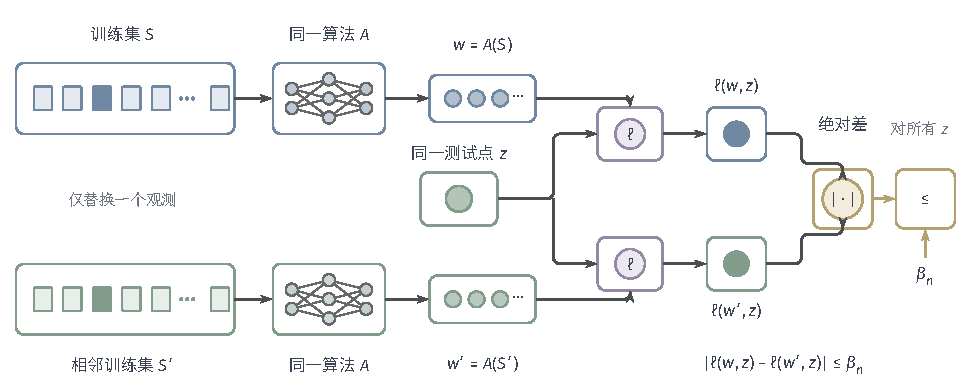
\includegraphics[width=164.600mm]{figures/03-foundations/02-learning-theory/tikz/learning-theory-stability/figure.pdf}
  \caption{算法稳定性的相邻样本实验。两批样本只替换一个观测，同一算法分别输出
  $\bm w=A(S)$与$\bm w'=A(S')$。两次输出在同一测试点$z$上计算损失，再比较绝对差；
  均匀稳定性要求所有这样的损失差都不超过$\beta_n$。图中的比较对象是损失，不是参数距离。}
  \label{fig:learning-stability}
\end{figure*}

因为要控制任意一种单项替换，上界必须同时对所有相邻样本和所有测试观测成立，这就是“均匀”的含义。

\begin{definition}[均匀稳定性]
\label{def:uniform-stability}
若对任意相邻$S,S'$和任意$z\in Z$都有
\begin{equation}
 |\ell(A(S),z)-\ell(A(S'),z)|\leq\beta_n,
 \label{eq:uniform-stability}
\end{equation}
则称算法$A$具有$\beta_n$均匀稳定性。
\end{definition}

定义中固定样本量$n$，把$A_n$简记为$A$。均匀稳定性只比较算法在相邻样本上实际产生的两个输出的损失，是对算法的要求；一致收敛则要估计整个决策空间的风险，是对空间的要求。两者控制的对象不同。

替换保持样本量$n$不变，删除把样本量变为$n-1$，所以替换稳定性与删除稳定性不能直接互推。例如，算法按样本量的奇偶输出两个不同常量：替换一项不改变样本量，输出不变；删除一项使样本量奇偶改变，输出可能跳变。反过来，如果另有一种对任意测试观测成立的均匀删除稳定性——删除任意一项后的输出与原输出在任意测试点上损失差至多$\beta_n^{\mathrm{del}}$——那么两份相邻样本都删去被替换的位置后，变成同一份$n-1$项样本；经这份共同样本比较两次输出，三角不等式给出替换稳定性上界$2\beta_n^{\mathrm{del}}$。

继续用$z_i\in[0,1]$的样本均值$A(S)=\bar z$，这次考察替换。替换一项后两个均值至多相差$1/n$；对绝对损失$\ell(w,z)=|w-z|$，在同一个测试观测$z$处，由反三角不等式有
\[
 \bigl||\bar z-z|-|\bar z'-z|\bigr|\leq|\bar z-\bar z'|\leq\frac1n.
\]
这个界对所有相邻样本和测试点同时成立，所以均值算法具有$1/n$均匀稳定性。它与前面的删除例子分别检验两种扰动；两者都没有证明均值使绝对损失最小，经验优化误差仍需单独检查。

\begin{theorem}[均匀稳定性与期望风险]
\label{thm:stability-expected-generalization}
设$(Z,\mathcal Z)$与$(\mathcal W,\mathcal B_{\mathcal W})$为可测空间，
$\ell:\mathcal W\times Z\to\mathbb R$可测，$\mathcal P$为$Z$上的概率分布，
$S=(z_1,\ldots,z_n)\sim\mathcal P^n$，且确定性算法
$A:Z^n\to\mathcal W$可测。令$z_i'\sim\mathcal P$独立于$S$，并以
$S^{(i)}$表示用$z_i'$替换$z_i$所得的样本。定义
\[
 R_{\mathcal P}(w)=\mathbb E_{z\sim\mathcal P}\ell(w,z),
 \qquad
 \hat R_S(w)=\frac1n\sum_{i=1}^n\ell(w,z_i).
\]
假定
$\ell(A(S),z_i)$、$\ell(A(S),z_i')$和$\ell(A(S^{(i)}),z_i')$均可积。
若任意只相差一个观测的$s,s'\in Z^n$及任意$z\in Z$都满足
\[
 |\ell(A(s),z)-\ell(A(s'),z)|\leq\beta_n,
\]
则
\begin{equation}
 \left|\mathbb E_S\left[R_{\mathcal P}(A(S))-\hat R_S(A(S))\right]\right|
 \leq\beta_n.
 \label{eq:stability-expectation-bound}
\end{equation}
\end{theorem}

\begin{proof}
取与$S$独立的$z_i'\sim\mathcal P$，令$S^{(i)}$把$z_i$替换为$z_i'$。交换$z_i$与$z_i'$不改变
全部独立观测的联合分布，因而$(S,z_i)$与$(S^{(i)},z_i')$同分布。
把函数$(s,z)\mapsto\ell(A(s),z)$分别作用于这两组同分布的变量，得到
$\mathbb E\ell(A(S),z_i)=\mathbb E\ell(A(S^{(i)}),z_i')$，所以经验风险的第$i$项可写成后者。
另一方面，$z_i'$独立于$S$，对它先取期望得到$R_{\mathcal P}(A(S))$，故期望风险项为
$\mathbb E\ell(A(S),z_i')$。两项都在同一个$z_i'$上评价，只是训练样本相差一项，因此
\begin{align*}
 &\mathbb E_S[R_{\mathcal P}(A(S))-\hat R_S(A(S))]\\
 &=\frac1n\sum_i\mathbb E
   [\ell(A(S),z_i')-\ell(A(S^{(i)}),z_i')]
 \leq\beta_n.
\end{align*}
交换$S$与$S^{(i)}$得到反向界。

\end{proof}

这个交换论证让$z_i'$同时扮演两个角色：对$A(S)$它是独立测试点，对$A(S^{(i)})$它是训练点。均匀稳定性保证同一个$z_i'$上两次输出的损失差很小，于是测试评价与训练评价接近。整个论证只使用算法的实际输出，没有对整个决策空间取上确界，这正是稳定性路线与一致收敛的区别。

式~\eqref{eq:stability-expectation-bound}中的绝对值在期望外面，因此不同样本上泛化差为正或负可以相互抵消；它既不是绝对泛化差的平均值，也不保证每份样本上泛化差都小。若算法随机化为$A(S,U)$，采用先对内部随机性取平均的定义：
\[
 \sup_{S,S'\text{相邻},\,z\in Z}
 \left|\mathbb E_U\ell(A(S,U),z)-\mathbb E_U\ell(A(S',U),z)\right|\leq\beta_n.
\]
其中$U$与样本独立，且对每个固定的$S,z$，$\ell(A(S,U),z)$关于$U$可积。把确定性算法的证明再对$U$平均，就控制了样本和内部随机性共同平均下的泛化差，但不保证每次随机运行都稳定。留一法稳定性也可以先对内部随机性平均，再比较删除前后的损失绝对差，其风险恒等式和学习保证同样成立。

上述上界控制的是经验评价的平均偏差。要判断算法是否学到了低风险决策，还需控制经验优化误差。若输出属于$\mathcal W$，且期望经验优化误差至多$\rho_n$，在定理~\ref{thm:generalization-optimization-learning}中令$g_n=\beta_n$，就得到$\beta_n+\rho_n$的平均超额风险界和相应的PAC保证。仅有$\beta_n\to0$而经验风险始终远离最优值，仍不能完成学习。这里的结论是验证某个算法的充分条件，还没有要求每个成功算法都必须均匀稳定。

如果只想在给定的一份样本上用经验风险估计期望风险，而暂不与最优决策比较，就需要控制泛化差在样本间的随机波动。损失有界且算法均匀稳定时，替换一项对泛化差的影响有统一上界，因此可以用有界差分不等式。下面先对确定性算法单独处理样本随机性。

\begin{theorem}[均匀稳定性的高概率泛化界]
\label{thm:stability-high-probability}
设$(Z,\mathcal Z)$与$(\mathcal W,\mathcal B_{\mathcal W})$为可测空间，
$\ell:\mathcal W\times Z\to[0,1]$可测，$\mathcal P$为$Z$上的概率分布，
$S=(z_1,\ldots,z_n)\sim\mathcal P^n$，且确定性算法
$A:Z^n\to\mathcal W$可测。定义
\[
 R_{\mathcal P}(w)=\mathbb E_{z\sim\mathcal P}\ell(w,z),
 \qquad
 \hat R_S(w)=\frac1n\sum_{i=1}^n\ell(w,z_i).
\]
若任意只相差一个观测的$s,s'\in Z^n$及任意
$z\in Z$都满足
\[
 |\ell(A(s),z)-\ell(A(s'),z)|\leq\beta_n,
\]
则任意$\delta\in(0,1)$下，以至少$1-\delta$的样本概率，有
\[
 |R_{\mathcal P}(A(S))-\hat R_S(A(S))|
 \leq\beta_n+(2n\beta_n+1)\sqrt{\frac{\log(2/\delta)}{2n}}.
\]
\end{theorem}
\begin{proof}
记$g(S)=R_{\mathcal P}(A(S))-\hat R_S(A(S))$。
替换一个观测后，期望风险变化至多$\beta_n$；经验风险的$n-1$个共同观测各变化至多
$\beta_n$，被替换项变化至多1。因此
$|g(S)-g(S')|\leq2\beta_n+1/n$。
对$n$个独立观测应用有界差分不等式，$g(S)$偏离其期望的绝对值以至少$1-\delta$的概率
不超过$(2n\beta_n+1)\sqrt{\log(2/\delta)/(2n)}$。
再使用$|\mathbb E g(S)|\leq\beta_n$即得结论。
\end{proof}

右侧第二项约为$2\beta_n\sqrt{n\log(2/\delta)/2}+\sqrt{\log(2/\delta)/(2n)}$。当$\beta_n=O(1/n)$时，第一部分为$O(1/\sqrt n)$，整个界随$n$增大趋于零；但若只有$\beta_n=1/\sqrt n$，第一部分不再下降，界失去作用。原因在于证明中每次替换使泛化差至多改变$2\beta_n+1/n$，有界差分不等式把$n$个这样的量平方相加，$\beta_n$必须远小于$1/\sqrt n$才能被吸收。更精细的集中分析给出
\[
 |R_{\mathcal P}(A(S))-\hat R_S(A(S))|
 \leq C\!\left(\beta_n\log(2n)\log\frac2\delta
          +\sqrt{\frac{\log(2/\delta)}n}\right),
\]
其中$C$是通用常数。这是Bousquet、Klochkov与Zhivotovskiy的高概率结果，其高阶矩证明不在本章展开\scite{bousquet2020sharper}。对随机算法，可以把该结论用于内部随机性平均后的损失；若要评价单次随机运行的输出，还需另外控制内部随机性造成的波动。

前面解决的是“给定一个算法，怎样验证它能学习”。反过来问：只要问题可学习，能否构造出一个既稳定、经验风险又接近最优的算法？回答这个问题时，要把经验最优性加强为对每份样本都成立，而不只是平均成立。

\begin{definition}[始终渐近经验风险最小化]
\label{def:aerm}
设随机算法$A(S,U)$的输出属于$\mathcal W$，$U$独立于样本。
若存在$\rho_n\to0$，使任意$S\in Z^n$均满足
\[
 \mathbb E_U\hat R_S(A(S,U))-\inf_{w\in\mathcal W}\hat R_S(w)\leq\rho_n,
\]
则称$A$为始终渐近经验风险最小化算法（always AERM）。
\end{definition}

“始终”限定的对象是样本：每一份样本都必须满足同一个$\rho_n$上界，只对内部随机性取平均。若先对允许分布下的样本取期望后才满足不依赖分布的速率，则称为在允许分布族上统一的AERM，条件较弱。“渐近”指允许经验风险略高于最低值，只要差距随样本量趋于零；这比精确ERM宽松，也恰好容纳了只求近似解的算法。下面采用更强的始终AERM，把稳定算法的存在性与可学习性联系起来\scite{shalevshwartz2010learnability}。

定理的读法可以与二分类对照。二分类中，可学习、VC维有限与一致收敛三者等价，一致收敛是可学习问题的共同性质。上一节已经说明，一般损失下一致收敛不再是必要的；下面的定理说明，起这个作用的是“存在稳定且始终渐近经验最优的算法”。也就是说，在一般学习中，刻画可学习性的不再是决策空间的某种容量，而是某个算法的行为。

\begin{theorem}[一般学习基本定理：均匀稳定性与可学习性]
\label{thm:general-stability-characterization}
设$(Z,\mathcal Z)$与$(\mathcal W,\mathcal B_{\mathcal W})$为可测空间，
$\mathcal W$非空，$\ell:\mathcal W\times Z\to[0,1]$可测，并允许$Z$上的所有
概率分布。对每个$n$，假定
$s\mapsto\inf_{w\in\mathcal W}n^{-1}\sum_{i=1}^n\ell(w,z_i)$可测；
随机算法均由可测映射$A_n:Z^n\times\mathcal U\to\mathcal W$表示，其内部随机数
$U$与样本$S\sim\mathcal P^n$独立。定义
\[
 R_{\mathcal P}(w)=\mathbb E_{z\sim\mathcal P}\ell(w,z),
 \qquad
 \hat R_S(w)=\frac1n\sum_{i=1}^n\ell(w,z_i).
\]
则以下两个命题等价：
\begin{enumerate}
 \item 存在随机算法$(B_n)$，使任意$\varepsilon,\delta\in(0,1)$都有不依赖
 $\mathcal P$的$n_0(\varepsilon,\delta)$，并且所有$n\geq n_0$均满足
 \[
  \mathbb P_{S,U}\!\left\{
  R_{\mathcal P}(B_n(S,U))-\inf_{w\in\mathcal W}R_{\mathcal P}(w)
  \leq\varepsilon\right\}\geq1-\delta
 \]
 对每个$Z$上的概率分布$\mathcal P$成立；
 \item 存在随机算法$(A_n)$及不依赖$\mathcal P$的非负序列
 $\rho_n\to0$、$\beta_n\to0$，使每份$s\in Z^n$都满足
 \[
  \mathbb E_U\hat R_s(A_n(s,U))
  -\inf_{w\in\mathcal W}\hat R_s(w)\leq\rho_n,
 \]
 而任意只相差一个观测的$s,s'\in Z^n$及任意$z\in Z$都满足
 \[
  \left|\mathbb E_U\ell(A_n(s,U),z)
  -\mathbb E_U\ell(A_n(s',U),z)\right|\leq\beta_n.
 \]
\end{enumerate}
\end{theorem}
\begin{proof}
命题2蕴含命题1：定理~\ref{thm:stability-expected-generalization}给出
$g_n=\beta_n$的期望泛化差上界，再由
定理~\ref{thm:generalization-optimization-learning}得到PAC保证。

逆向从已有学习算法$B$出发。构造的想法是：只让$B$看样本中随机抽出的一小部分。抽出的项数$k$要随$n$增长，$B$才能学好；又要满足$k/n\to0$，被替换的那一项才很少被看到，输出才稳定。$k=\lfloor\sqrt n\rfloor$同时满足两点。下面先把$B$的PAC保证改写成随样本量趋于零的期望界，再验证这两点。因为损失有界，我们可将超额期望风险按PAC成功和失败事件分开：成功时至多$\varepsilon$，失败时至多1，故期望至多$\varepsilon+\delta$。PAC保证对每一对$(\varepsilon,\delta)$各给一个样本量门槛，而后面的构造需要一列随样本量$k$趋于零、且不依赖分布的期望界$a_k$，下面把这些门槛拼接起来。具体地，对每个整数$r\geq1$，由PAC保证选择门槛$N_r$，使$k\geq N_r$时取$\varepsilon=\delta=1/r$可得期望超额风险至多$2/r$。再令$N'_r=\max\{r,N_1,\ldots,N_r\}$；这组门槛单调且满足$N'_r\geq r$，所以集合$\{r:N'_r\leq k\}$有限。该集合非空时，令$r(k)$为其中的最大等级并取$a_k=2/r(k)$；在它为空的有限前缀取平凡界$a_k=1$。任意固定等级最终都会进入集合，故$r(k)\to\infty$、$a_k\to0$，而这个平均超额风险上界对允许分布统一成立。

利用$B$构造新的算法。对输入$S$，有放回地独立抽取$k=\lfloor\sqrt n\rfloor$个位置$J=(J_1,\ldots,J_k)$，将对应序列$T$交给$B$。若$B$还使用随机数$U_0$，新算法的随机数就是$U=(J,U_0)$。固定$S$后，$T$独立取自经验分布$\mathcal P_S=n^{-1}\sum_i\delta_{z_i}$，其中$\delta_{z_i}$为点质量分布。由于$R_{\mathcal P_S}(w)=\hat R_S(w)$，$B$在这一分布上的学习保证给出
\[
 \mathbb E_{J,U_0}\hat R_S(B(T,U_0))-\inf_w\hat R_S(w)\leq a_k.
\]
经验分布可以来自任意$S$，因此新算法对每份样本都满足AERM，且$\rho_n=a_k\to0$。

在相邻样本上共享索引$J$及随机数$U_0$，两次输出只有访问被替换位置时才可能不同。访问该位置的概率至多$k/n$，损失变化至多1，所以$\beta_n\leq k/n\to0$。构造的算法同时满足稳定性与始终AERM，逆向因此成立。
\end{proof}

必要性的证明构造了一个新的算法，说明可学习时存在一个稳定的学习算法，并不证明原来的每个成功算法都稳定。有放回子采样的构造也只用于存在性证明，没有追求最优的样本效率或计算效率。

\subsection{平均稳定性}
\label{sec:on-average-stability}

均匀稳定性要求最不利的样本替换也只有很小影响，而期望泛化差只涉及随机抽样后的平均影响。若少数样本引起的变化很大，但这些样本出现的概率很低，均匀上界可能过于保守。因此我们保持替换方式不变，改为直接计算损失变化的平均值，以保留数据分布的信息。

仍令$S=(z_1,\ldots,z_n)\sim\mathcal P^n$，用独立的$z_i'\sim\mathcal P$替换$z_i$得到$S^{(i)}$，这次在被替换出去的$z_i$上评价。$A(S)$在训练中见过$z_i$，$A(S^{(i)})$没见过它，二者在$z_i$上的损失差衡量“用$z_i$训练”在该观测上带来的平均优势。对样本、替换观测和位置取平均，得到\term{平均稳定性}（on-average stability）。这里采用一侧的平均替换定义，与《Understanding Machine Learning》第13章的约定一致\scite{shalevshwartz2014}。

\begin{definition}[平均稳定性]
\label{def:on-average-stability}
设$U$为独立于所有观测的算法内部随机数，并满足稳定性可积性条件。定义
\begin{equation}
 \gamma_n(A,\mathcal P)
 =\frac1n\sum_{i=1}^n\mathbb E_{S,z_i',U}
 \left[\ell(A(S^{(i)},U),z_i)-\ell(A(S,U),z_i)\right].
 \label{eq:on-average-stability}
\end{equation}
给定$\bar\beta_n(\mathcal P)\geq0$，若
$\gamma_n(A,\mathcal P)\leq\bar\beta_n(\mathcal P)$，则称算法在分布$\mathcal P$下具有
速率$\bar\beta_n(\mathcal P)$的平均稳定性。
若对所有允许分布均有$\gamma_n(A,\mathcal P)\leq\bar\beta_n$，且$\bar\beta_n$不依赖
$\mathcal P$，则称算法具有速率$\bar\beta_n$的在允许分布族上统一的平均稳定性。
\end{definition}

确定性算法可省略$U$。定义只要求上界而不要求绝对值，是因为学习保证只需防止经验风险低估期望风险；若经验评价反而偏高，风险分解中的相应项为负，只会使上界更松而不会失效。这个定义取有符号损失差的平均，不同样本上的增加和减少可以抵消；它只限制平均意义下训练带来的优势，不限制每次替换的绝对变化。先对每项取绝对值再平均是更强的要求。均匀稳定性蕴含这里的平均条件，反方向一般不成立。与平均留一法相比，这里两次训练都使用$n$项样本，而留一法联系的是$n$项与$n-1$项算法。

\begin{theorem}[平均稳定性与期望风险]
\label{thm:on-average-generalization}
设$(Z,\mathcal Z)$与$(\mathcal W,\mathcal B_{\mathcal W})$为可测空间，
$\ell:\mathcal W\times Z\to\mathbb R$可测，$\mathcal P$为$Z$上的概率分布。
令$S=(z_1,\ldots,z_n)\sim\mathcal P^n$，令
$z_1',\ldots,z_n'\sim\mathcal P$彼此独立并独立于$S$，以$S^{(i)}$表示用
$z_i'$替换$z_i$所得的样本。令算法内部随机数$U$独立于所有观测，且可测算法
$A:Z^n\times\mathcal U\to\mathcal W$输出$A(S,U)$。再令
$z\sim\mathcal P$独立于$S,U,z_1',\ldots,z_n'$。假定
$\ell(A(S,U),z_i)$、$\ell(A(S^{(i)},U),z_i)$以及独立测试损失
$\ell(A(S,U),z)$均可积。定义
\[
 R_{\mathcal P}(w)=\mathbb E_{z\sim\mathcal P}\ell(w,z),
 \qquad
 \hat R_S(w)=\frac1n\sum_{i=1}^n\ell(w,z_i),
\]
并定义
\[
 \gamma_n(A,\mathcal P)
 =\frac1n\sum_{i=1}^n\mathbb E_{S,z_i',U}
 \left[\ell(A(S^{(i)},U),z_i)-\ell(A(S,U),z_i)\right].
\]
则
\begin{equation}
 \mathbb E_{S,U}\left[R_{\mathcal P}(A(S,U))-\hat R_S(A(S,U))\right]
 =\gamma_n(A,\mathcal P).
 \label{eq:on-average-generalization-identity}
\end{equation}
因此，若$\bar\beta_n(\mathcal P)\geq0$且
$\gamma_n(A,\mathcal P)\leq\bar\beta_n(\mathcal P)$，则
\[
 \mathbb E_{S,U}R_{\mathcal P}(A(S,U))
 \leq\mathbb E_{S,U}\hat R_S(A(S,U))+\bar\beta_n(\mathcal P).
\]
\end{theorem}
\begin{proof}
替换后，$S^{(i)}$仍由$n$个独立同分布的观测组成，而且独立于被替换出去的$z_i$。
在给定$S^{(i)}$和$U$时，对$z_i$取期望得到
\[
 \mathbb E_{z_i}\ell(A(S^{(i)},U),z_i)
 =R_{\mathcal P}(A(S^{(i)},U)).
\]
再利用$S^{(i)}$与$S$同分布，得到
$\mathbb E\ell(A(S^{(i)},U),z_i)=\mathbb E_{S,U}R_{\mathcal P}(A(S,U))$。
另一方面，$n$个原观测上的损失平均恰好是经验风险，故
\[
 \frac1n\sum_{i=1}^n\mathbb E_{S,U}\ell(A(S,U),z_i)
 =\mathbb E_{S,U}\hat R_S(A(S,U)).
\]
两式相减即得恒等式，再代入平均稳定性上界，得到期望风险的上界。
\end{proof}

恒等式说明，平均替换分析的直接对象就是期望风险与经验风险之差的平均值：为正表示经验评价平均偏低，为负表示平均偏高。这是多次抽样并重新训练后的平均关系；单次训练的泛化差仍可能很大，绝对差的平均值也未必小。若速率只对某个固定分布$\mathcal P$成立，结论也只限于该分布；允许族上的统一学习还要求上界对该族内所有分布统一；要称为分布无关学习，还须允许全部相关分布。

现在把平均稳定性与经验优化误差合并。设$A(S,U)\in\mathcal W$具有在允许分布族上统一的平均稳定性上界$\bar\beta_n$，并且平均经验优化误差满足
\[
 \mathbb E_{S,U}[\hat R_S(A(S,U))-\inf_w\hat R_S(w)]\leq\rho_n.
\]
把定理~\ref{thm:on-average-generalization}给出的$g_n=\bar\beta_n$代入定理~\ref{thm:generalization-optimization-learning}，得到
\begin{equation}
 \mathbb E_{S,U}R_{\mathcal P}(A(S,U))-
 \inf_{w\in\mathcal W}R_{\mathcal P}(w)\leq\bar\beta_n+\rho_n.
 \label{eq:stability-excess-risk}
\end{equation}
当$\bar\beta_n\to0$且$\rho_n\to0$时，算法PAC学习该问题；条件$\bar\beta_n+\rho_n\leq\varepsilon\delta$保证超额期望风险超过$\varepsilon$的概率不超过$\delta$。

由平均界转成概率结论时，Markov不等式只能用于非负的超额期望风险，不能直接用于有符号的泛化差。固定分布下的速率只给出该分布下的保证；稳定性速率和经验优化误差上界若在允许族上统一，才得到相对于该族的统一PAC结论；允许族包含全部相关分布时，结论才是分布无关的。

用均值估计的例子可以直接算出这种分布依赖。设$z\in[0,1]$的均值为$\mu$、方差为$\sigma^2$，算法输出样本均值$\bar z$，这次用平方损失$\ell(w,z)=(w-z)^2$评价。对独立观测有$R_{\mathcal P}(\bar z)=\sigma^2+(\bar z-\mu)^2$，所以
\[
 \mathbb E_S R_{\mathcal P}(\bar z)=\sigma^2+\frac{\sigma^2}{n}.
\]
经验风险可用恒等式$\sum_i(z_i-\bar z)^2=\sum_i(z_i-\mu)^2-n(\bar z-\mu)^2$计算其期望，得到
\[
 \mathbb E_S\hat R_S(\bar z)=\sigma^2-\frac{\sigma^2}{n},
 \qquad \gamma_n(A,\mathcal P)=\frac{2\sigma^2}{n}.
\]
方差越小，平均替换带来的损失变化越小；观测恒定时$\sigma^2=0$，该量为零。只知道取值范围时，由$\sigma^2\leq1/4$得到分布无关上界$1/(2n)$。另一方面，对$w,w',z\in[0,1]$有$|(w-z)^2-(w'-z)^2|=|w-w'||w+w'-2z|\leq2|w-w'|$，替换使均值移动至多$1/n$，故均匀稳定性上界为$2/n$。平均分析利用了最坏情形分析没有使用的方差信息。样本均值恰好是平方损失的经验最优解，所以$\rho_n=0$，稳定性方法给出平均超额风险至多$2\sigma^2/n$；直接计算得到精确值$\mathbb E(\bar z-\mu)^2=\sigma^2/n$，二者同阶，但稳定性常数较宽松。由方差界，$n\geq1/(2\varepsilon\delta)$足以满足这条分析给出的PAC要求。

平均条件弱于均匀条件，但在讨论算法存在性时，二者给出相同的可学习性刻画，下一个定理说明这一点。

\begin{theorem}[一般学习基本定理的平均稳定性形式]
\label{thm:average-stability-characterization}
设$(Z,\mathcal Z)$与$(\mathcal W,\mathcal B_{\mathcal W})$为可测空间，
$\mathcal W$非空，$\ell:\mathcal W\times Z\to[0,1]$可测，并允许$Z$上的所有
概率分布。对每个$n$，假定
$s\mapsto\inf_{w\in\mathcal W}n^{-1}\sum_{i=1}^n\ell(w,z_i)$可测；
随机算法均由可测映射$A_n:Z^n\times\mathcal U\to\mathcal W$表示，其内部随机数
$U$与全部观测独立。令$S=(z_1,\ldots,z_n)\sim\mathcal P^n$，
令$z_i'\sim\mathcal P$独立于$S,U$，并以$S^{(i)}$表示用$z_i'$替换$z_i$所得样本。
定义
\[
\begin{aligned}
 R_{\mathcal P}(w)
 &=\mathbb E_{z\sim\mathcal P}\ell(w,z),\\
 \hat R_S(w)
 &=\frac1n\sum_{i=1}^n\ell(w,z_i),\\
 \gamma_n(A_n,\mathcal P)
 &=\frac1n\sum_{i=1}^n\mathbb E\!\left[
   \ell(A_n(S^{(i)},U),z_i)-\ell(A_n(S,U),z_i)\right].
\end{aligned}
\]
则该问题分布无关PAC可学习，也就是存在随机算法$(B_n)$，使任意
$\varepsilon,\delta\in(0,1)$都有不依赖$\mathcal P$的$n_0$，且所有$n\geq n_0$
均满足
\[
 \mathbb P_{S,U}\!\left\{
 R_{\mathcal P}(B_n(S,U))-\inf_{w\in\mathcal W}R_{\mathcal P}(w)
 \leq\varepsilon\right\}\geq1-\delta,
\]
当且仅当存在随机算法$(A_n)$以及不依赖$\mathcal P$的非负序列
$\rho_n\to0$、$\bar\beta_n\to0$，使每份$s\in Z^n$都满足
\[
 \mathbb E_U\hat R_s(A_n(s,U))
 -\inf_{w\in\mathcal W}\hat R_s(w)\leq\rho_n,
\]
并且每个$Z$上的概率分布$\mathcal P$都满足
\[
 \gamma_n(A_n,\mathcal P)\leq\bar\beta_n.
\]
\end{theorem}
\begin{proof}
充分性由定理~\ref{thm:on-average-generalization}与
定理~\ref{thm:generalization-optimization-learning}给出。
对于必要性，前面的基本定理保证可学习问题存在均匀稳定的始终AERM算法；
均匀稳定性又蕴含平均稳定性，因此同一个算法满足这里的条件。
\end{proof}

这里的等价是针对问题的：存在一组算法满足平均条件，与存在一组算法满足均匀条件相互等价，两边可以使用不同的算法。固定某一个算法后，平均稳定性不能升级为均匀稳定性，一侧的平均保证也不能升级为逐样本保证。

\subsection{参数稳定性}
\label{sec:parameter-stability}

损失稳定性直接比较损失，但正则化和梯度下降的分析通常先得到两次训练输出参数之间的距离，然后才估计损失差；因此需要第二类条件。\term{参数稳定性}（argument stability，也称model stability）直接控制这个距离。本小节令$\mathcal W\subseteq\mathbb R^d$，用欧氏范数度量参数向量；换一种参数表示或距离，条件本身也会改变。平均参数稳定性可以用于优化算法的精细泛化分析\scite{lei2020finegrained}。

\begin{definition}[均匀参数稳定性]
\label{def:uniform-parameter-stability}
设算法$A(S,U)\in\mathcal W\subseteq\mathbb R^d$。若对任意相邻样本$S,S'$都有
\[
 \mathbb E_U\|A(S,U)-A(S',U)\|_2\leq\alpha_n,
\]
则称算法具有速率$\alpha_n$的均匀参数稳定性。两次运行使用相同的内部随机数$U$。
\end{definition}

\begin{definition}[平均参数稳定性]
\label{def:average-parameter-stability}
沿用定义~\ref{def:on-average-stability}中的$S,S^{(i)}$和$U$。
若
\begin{equation}
 \frac1n\sum_{i=1}^n\mathbb E_{S,z_i',U}
 \|A(S,U)-A(S^{(i)},U)\|_2\leq\bar\alpha_n(\mathcal P),
 \label{eq:average-parameter-stability}
\end{equation}
则称算法在分布$\mathcal P$下具有速率$\bar\alpha_n(\mathcal P)$的平均参数稳定性。
若同一个上界适用于所有允许分布，则称其为在允许分布族上统一的平均参数稳定性。
\end{definition}

两次运行共享同一个内部随机数$U$，是为了排除算法自身随机性造成的差别。例如比较两次SGD时使用相同的初始化和样本索引序列，输出之差才反映样本替换的影响；若独立采样内部随机数，即使样本完全相同，输出也可能不同。均匀参数稳定性对每对相邻样本都控制参数距离；平均参数稳定性则按$\mathcal P$下样本出现的概率平均。

样本均值可以直接算出参数距离：替换一项后$A(S^{(i)})-A(S)=(z_i'-z_i)/n$。在$[0,1]$上，均匀界为$1/n$，平均界为$\mathbb E|z-z'|/n$。若$z$以概率$p$取1、其余取0，两次独立取值不同的概率为$2p(1-p)$，平均界为$2p(1-p)/n$。数据几乎恒定时，这个平均距离比最坏情形距离小得多。

参数距离本身不是风险量，要进入风险分析还需把它转换成损失变化。若存在常数$L$，使任意$\bm u,\bm v\in\mathcal W$和$z\in Z$都满足
\begin{equation}
 |\ell(\bm u,z)-\ell(\bm v,z)|\leq L\|\bm u-\bm v\|_2,
 \label{eq:parameter-loss-lipschitz}
\end{equation}
则称损失关于参数是$L$-Lipschitz的。它保证参数移动距离$r$时，同一观测上的损失至多改变$Lr$，因此参数稳定性可以接入前面的损失稳定性定理。

\begin{theorem}[参数稳定性与损失稳定性]
\label{thm:parameter-to-loss-stability}
设$(Z,\mathcal Z)$为可测观测空间，
$\mathcal W\subseteq\mathbb R^d$配备Borel $\sigma$代数，
$\ell:\mathcal W\times Z\to\mathbb R$可测，并且对任意
$\bm u,\bm v\in\mathcal W$及$z\in Z$都有
\[
 |\ell(\bm u,z)-\ell(\bm v,z)|
 \leq L\|\bm u-\bm v\|_2.
\]
令可测算法$A:Z^n\times\mathcal U\to\mathcal W$使用内部随机数$U$；
比较两份样本时，两次运行共享同一个$U$。假定每个固定$s\in Z^n,z\in Z$下，
$\ell(A(s,U),z)$关于$U$可积。若任意只相差一个观测的$s,s'\in Z^n$均满足
\[
 \mathbb E_U\|A(s,U)-A(s',U)\|_2\leq\alpha_n,
\]
则任意这样的$s,s'$及任意$z\in Z$均满足
\[
 \left|\mathbb E_U\ell(A(s,U),z)-\mathbb E_U\ell(A(s',U),z)\right|
 \leq L\alpha_n.
\]
另一方面，固定$Z$上的概率分布$\mathcal P$，令
$S=(z_1,\ldots,z_n)\sim\mathcal P^n$，令$z_i'\sim\mathcal P$独立于
$S,U$，并以$S^{(i)}$表示用$z_i'$替换$z_i$所得的样本。假定
$\ell(A(S,U),z_i)$与$\ell(A(S^{(i)},U),z_i)$均可积。若
\[
 \frac1n\sum_{i=1}^n\mathbb E_{S,z_i',U}
 \|A(S,U)-A(S^{(i)},U)\|_2
 \leq\bar\alpha_n(\mathcal P),
\]
则
\[
 \frac1n\sum_{i=1}^n\mathbb E_{S,z_i',U}
 [\ell(A(S^{(i)},U),z_i)-\ell(A(S,U),z_i)]
 \leq L\bar\alpha_n(\mathcal P).
\]
\end{theorem}
\begin{proof}
对任意相邻样本和任意观测，Lipschitz条件给出
\[
 \left|\mathbb E_U\ell(A(S,U),z)-\mathbb E_U\ell(A(S',U),z)\right|
 \leq L\mathbb E_U\|A(S,U)-A(S',U)\|_2.
\]
代入均匀参数稳定性上界得到第一项结论。
对于平均稳定性，对定义~\ref{def:on-average-stability}中的损失差逐项取绝对值，
再使用Lipschitz条件，得到
\[
 |\gamma_n(A,\mathcal P)|
 \leq\frac Ln\sum_{i=1}^n\mathbb E_{S,z_i',U}
       \|A(S^{(i)},U)-A(S,U)\|_2
 \leq L\bar\alpha_n(\mathcal P).
\]
这也给出了平均稳定性所需的一侧上界。
\end{proof}

完成这一转换后，参数化算法也能使用平均稳定性中的替换样本恒等式。这里仍要区分单次训练的泛化差$R_{\mathcal P}(A(S,U))-\hat R_S(A(S,U))$与对$S,U$平均后的期望泛化差：平均参数距离直接约束的是后者，即经验评价的平均偏差有多大。

\begin{theorem}[参数稳定性与期望泛化差]
\label{thm:parameter-expected-generalization}
设$(Z,\mathcal Z)$为可测观测空间，
$\mathcal W\subseteq\mathbb R^d$配备Borel $\sigma$代数，
$\ell:\mathcal W\times Z\to\mathbb R$可测，并且对任意
$\bm u,\bm v\in\mathcal W$及$z\in Z$都有
\[
 |\ell(\bm u,z)-\ell(\bm v,z)|
 \leq L\|\bm u-\bm v\|_2.
\]
固定$Z$上的概率分布$\mathcal P$，令
$S=(z_1,\ldots,z_n)\sim\mathcal P^n$，令算法内部随机数$U$独立于$S$，
并令可测算法$A:Z^n\times\mathcal U\to\mathcal W$输出$A(S,U)$。
令$z_i'\sim\mathcal P$独立于$S,U$，并以$S^{(i)}$表示用$z_i'$替换$z_i$
所得的样本；再令$z\sim\mathcal P$独立于$S,U,z_i'$。定义
\[
 R_{\mathcal P}(w)=\mathbb E_{z\sim\mathcal P}\ell(w,z),
 \qquad
 \hat R_S(w)=\frac1n\sum_{i=1}^n\ell(w,z_i).
\]
假定独立测试损失$\ell(A(S,U),z)$、训练损失
$\ell(A(S,U),z_i)$和替换损失$\ell(A(S^{(i)},U),z_i)$均可积。若
\[
 \frac1n\sum_{i=1}^n\mathbb E_{S,z_i',U}
 \|A(S,U)-A(S^{(i)},U)\|_2
 \leq\bar\alpha_n(\mathcal P),
\]
则
\begin{equation}
 \left|\mathbb E_{S,U}
 [R_{\mathcal P}(A(S,U))-\hat R_S(A(S,U))]\right|
 \leq L\bar\alpha_n(\mathcal P).
 \label{eq:parameter-generalization}
\end{equation}
特别地，期望风险满足
\[
 \mathbb E_{S,U}R_{\mathcal P}(A(S,U))
 \leq\mathbb E_{S,U}\hat R_S(A(S,U))+L\bar\alpha_n(\mathcal P).
\]
若任意只相差一个观测的$s,s'\in Z^n$都满足
$\mathbb E_U\|A(s,U)-A(s',U)\|_2\leq\alpha_n$，则可将两式中的
$\bar\alpha_n(\mathcal P)$替换为$\alpha_n$。
\end{theorem}
\begin{proof}
替换样本恒等式~\eqref{eq:on-average-generalization-identity}给出
\[
 \mathbb E_{S,U}[R_{\mathcal P}(A(S,U))-\hat R_S(A(S,U))]
 =\gamma_n(A,\mathcal P).
\]
前一定理的证明已经得到$|\gamma_n(A,\mathcal P)|\leq L\bar\alpha_n(\mathcal P)$，
故第一式成立。取其上侧不等式，并把平均经验风险移到右侧，即得第二式。
均匀参数稳定性对每对相邻样本都成立，对这些样本取平均后仍成立，故可取
$\bar\alpha_n(\mathcal P)\leq\alpha_n$。
\end{proof}

这个界先对泛化差取平均、再取绝对值，正负偏差仍可抵消，所以$L\bar\alpha_n(\mathcal P)$不能用于某一次训练的绝对泛化差。要在给定样本上由经验风险估计期望风险，可以加强为均匀参数稳定性，并限制损失的取值范围。

\begin{theorem}[均匀参数稳定性的高概率泛化界]
\label{thm:parameter-high-probability}
设$(Z,\mathcal Z)$为可测观测空间，
$\mathcal W\subseteq\mathbb R^d$配备Borel $\sigma$代数，
$\ell:\mathcal W\times Z\to[0,1]$可测，并且对任意
$\bm u,\bm v\in\mathcal W$及$z\in Z$都有
\[
 |\ell(\bm u,z)-\ell(\bm v,z)|
 \leq L\|\bm u-\bm v\|_2.
\]
固定$Z$上的概率分布$\mathcal P$，令
$S=(z_1,\ldots,z_n)\sim\mathcal P^n$，并令确定性可测算法
$A:Z^n\to\mathcal W$满足
\[
 \|A(s)-A(s')\|_2\leq\alpha_n
\]
对任意只相差一个观测的$s,s'\in Z^n$成立。定义
\[
 R_{\mathcal P}(w)=\mathbb E_{z\sim\mathcal P}\ell(w,z),
 \qquad
 \hat R_S(w)=\frac1n\sum_{i=1}^n\ell(w,z_i).
\]
对任意$\delta\in(0,1)$，以至少$1-\delta$的样本概率，有
\begin{align*}
 |R_{\mathcal P}(A(S))-\hat R_S(A(S))|
 \leq{}&L\alpha_n\\
 &+(2nL\alpha_n+1)\sqrt{\frac{\log(2/\delta)}{2n}}.
\end{align*}
\end{theorem}
\begin{proof}
由定理~\ref{thm:parameter-to-loss-stability}，该算法具有$L\alpha_n$均匀稳定性。
将$\beta_n=L\alpha_n$代入定理~\ref{thm:stability-high-probability}即得结论。
\end{proof}

$L$固定且$\alpha_n=O(1/n)$时，高概率界趋于零。仅有$\alpha_n\to0$还不足以保证该式下降，较慢的速率可能需要使用前面提到的精细集中结果。定义~\ref{def:uniform-parameter-stability}对随机算法只平均内部随机数，因而分析的是内部随机性平均后的损失；单次随机输出的风险还需另外控制。

参数稳定并不保证算法选到了低风险决策。前面“观测恒为1、算法始终输出0”的例子中，输出不随样本变化，参数稳定性常数为零，算法却远离最优决策。因此学习保证还必须单独约束经验优化误差。

\begin{theorem}[参数稳定性与可学习性]
\label{thm:parameter-stability-learning}
设$(Z,\mathcal Z)$为可测观测空间，
$\mathcal W\subseteq\mathbb R^d$为非空Borel决策空间，
$\ell:\mathcal W\times Z\to\mathbb R$可测，并且对任意
$\bm u,\bm v\in\mathcal W$及$z\in Z$都有
\[
 |\ell(\bm u,z)-\ell(\bm v,z)|
 \leq L\|\bm u-\bm v\|_2,
\]
其中$L$不依赖分布或样本量。对每个允许分布$\mathcal P$，令
$S=(z_1,\ldots,z_n)\sim\mathcal P^n$，令算法内部随机数$U$独立于$S$，
并令可测算法$A:Z^n\times\mathcal U\to\mathcal W$输出$A(S,U)$。
令$z_i'\sim\mathcal P$独立于$S,U$，并以$S^{(i)}$表示用$z_i'$替换$z_i$
所得的样本；再令$z\sim\mathcal P$独立于$S,U,z_i'$。定义
\[
 R_{\mathcal P}(\bm w)=\mathbb E_{z\sim\mathcal P}\ell(\bm w,z),
 \qquad
 \hat R_S(\bm w)=\frac1n\sum_{i=1}^n\ell(\bm w,z_i).
\]
假定独立测试损失、训练损失、替换损失以及每个固定
$\bm w\in\mathcal W$的$\ell(\bm w,z)$均可积；出现的经验风险和期望风险下确界
为有限实数且可测。若存在不依赖$\mathcal P$的非负数$\bar\alpha_n,\rho_n$，使
\[
 \frac1n\sum_{i=1}^n\mathbb E_{S,z_i',U}
 \|A(S,U)-A(S^{(i)},U)\|_2\leq\bar\alpha_n
\]
并且
\[
 \mathbb E_{S,U}\!\left[\hat R_S(A(S,U))-
 \inf_{\bm w\in\mathcal W}\hat R_S(\bm w)\right]\leq\rho_n,
\]
其中$\bar\alpha_n,\rho_n$均不依赖分布，则
\[
 \mathbb E_{S,U}R_{\mathcal P}(A(S,U))-
 \inf_{\bm w\in\mathcal W}R_{\mathcal P}(\bm w)
 \leq L\bar\alpha_n+\rho_n.
\]
若$\bar\alpha_n\to0$且$\rho_n\to0$，则算法相对于允许族$\mathfrak P$统一地PAC学习此问题；允许族包含全部相关分布时才称为分布无关PAC学习。
具体地，$L\bar\alpha_n+\rho_n\leq\varepsilon\delta$是达到精度$\varepsilon$与
置信度$1-\delta$的充分样本量条件。若任意只相差一个观测的$s,s'\in Z^n$都满足
$\mathbb E_U\|A(s,U)-A(s',U)\|_2\leq\alpha_n$，则可用$\alpha_n$替换
$\bar\alpha_n$。
\end{theorem}
\begin{proof}
定理~\ref{thm:parameter-expected-generalization}给出
$g_n=L\bar\alpha_n$的期望泛化差上界。将它与题设的经验优化误差代入
定理~\ref{thm:generalization-optimization-learning}即得全部结论。
\end{proof}

本定理通过非负的超额期望风险完成概率转换，与前一个高概率泛化界的集中证明不同。因此只要稳定性代价和经验优化误差两项都趋于零，就能得到学习保证，不必先证明前一个高概率界下降。固定分布下的两项上界只给出该分布的结论；允许族上的统一结论要求两项速率对该族内所有分布统一；分布无关结论还要求允许全部相关分布。

继续用Bernoulli观测的例子：$z$以概率$p$取1、其余取0，$\mathcal W=[0,1]$，用平方损失评价样本均值。这里$L=2$、平均参数距离$\bar\alpha_n(\mathcal P)=2p(1-p)/n$，且均值是经验最优解，故$\rho_n=0$。分别代入定理~\ref{thm:parameter-expected-generalization}和定理~\ref{thm:parameter-stability-learning}，得到
\begin{align*}
 \left|\mathbb E[R_{\mathcal P}(\bar z)-\hat R_S(\bar z)]\right|
 &\leq\frac{4p(1-p)}n,\\
 \mathbb E R_{\mathcal P}(\bar z)-\inf_{w\in[0,1]}R_{\mathcal P}(w)
 &\leq\frac{4p(1-p)}n.
\end{align*}
同一个右侧，在第一式中约束经验评价与总体评价的偏差，在第二式中约束输出与最优决策的差距。由$p(1-p)\leq1/4$，可取分布无关的充分样本量$n\geq1/(\varepsilon\delta)$。这比直接按损失变化平均得到的常数宽松，因为统一的Lipschitz转换没有保留平方损失的具体结构。

参数距离小并不自动意味着损失变化小。对阈值分类器$h_w(x)=\mathbb I\{x\geq w\}$，参数从$-a$移到$a$只移动$2a$，但在$(x,y)=(0,1)$处，零一损失对任意$a>0$都从0跳为1。反方向也不成立：若损失为$\ell((a,b),z)=(a-z)^2$，参数$b$完全不影响损失，任意改变$b$损失都不变。因此参数稳定性依赖于参数表示和距离的选择，它是一条充分的分析路径，不是每个成功算法都必须满足的性质。

Lipschitz条件并不总能满足。以一维平方损失$\ell(w,z)=(w-z)^2/2$为例，梯度为$w-z$：残差为1时参数移动0.01，损失约变化0.01；残差为100时，同样的移动使损失约变化1。参数无界时残差可以任意大，找不到统一的Lipschitz常数。不过，两处梯度之差恰为$u-v$，梯度的变化速度是固定的。这提示我们改用光滑性（smoothness）：若$\|\nabla\ell(\bm u,z)-\nabla\ell(\bm v,z)\|_2\leq M\|\bm u-\bm v\|_2$，称损失为$M$-光滑，即梯度随参数的变化不超过速率$M$。

光滑性本身不限制梯度大小，还需要借助损失非负这一条件。非负光滑损失满足自界关系$\|\nabla\ell(\bm u,z)\|_2^2\leq2M\ell(\bm u,z)$：损失小的地方，梯度也必然小，因为若梯度很大，沿负梯度走一小步就会使损失降到零以下。这样，梯度项可以用训练损失控制。推导中还会出现距离的平方，所以需要把平均参数距离加强为均方根距离：
\[
 b_n^2(\mathcal P)
 =\frac1n\sum_{i=1}^n\mathbb E_{S,z_i',U}
       \|A(S^{(i)},U)-A(S,U)\|_2^2.
\]
其中$b_n(\mathcal P)$先对参数距离的平方取平均，再开平方。由Cauchy--Schwarz不等式，它不小于平均参数距离，所以限制均方根距离是一项更强的要求。下一个定理不再假定梯度在所有参数处都有同一个有限上界，而是用训练损失的平均值来控制证明中出现的梯度项。

\begin{theorem}[光滑损失下参数稳定性与期望泛化差]
\label{thm:smooth-parameter-generalization}
设$(Z,\mathcal Z)$为可测观测空间，$\mathcal W=\mathbb R^d$，
$\ell:\mathbb R^d\times Z\to[0,\infty)$可测。对任意$z$，
$\ell(\cdot,z)$在$\mathbb R^d$上可微且$M$-光滑，其中$M>0$，即
\[
 \|\nabla\ell(\bm u,z)-\nabla\ell(\bm v,z)\|_2
 \leq M\|\bm u-\bm v\|_2.
\]
固定$Z$上的概率分布$\mathcal P$，令
$S=(z_1,\ldots,z_n)\sim\mathcal P^n$，令算法内部随机数$U$独立于$S$，
并令可测算法$A:Z^n\times\mathcal U\to\mathbb R^d$输出$A(S,U)$。
令$z_i'\sim\mathcal P$独立于$S,U$，并以$S^{(i)}$表示用$z_i'$替换$z_i$
所得的样本；再令$z\sim\mathcal P$独立于$S,U,z_i'$。定义
\[
 R_{\mathcal P}(\bm w)=\mathbb E_{z\sim\mathcal P}\ell(\bm w,z),
 \qquad
 \hat R_S(\bm w)=\frac1n\sum_{i=1}^n\ell(\bm w,z_i).
\]
假定独立测试损失$\ell(A(S,U),z)$、训练损失
$\ell(A(S,U),z_i)$和替换损失$\ell(A(S^{(i)},U),z_i)$均可积。定义
\[
 b_n^2(\mathcal P)
 =\frac1n\sum_{i=1}^n\mathbb E_{S,z_i',U}
 \|A(S^{(i)},U)-A(S,U)\|_2^2,
\]
并假定$b_n(\mathcal P)<\infty$。记
$r_n=\mathbb E_{S,U}\hat R_S(A(S,U))<\infty$。则
\begin{equation}
 \mathbb E_{S,U}[R_{\mathcal P}(A(S,U))-\hat R_S(A(S,U))]
 \leq b_n(\mathcal P)\sqrt{2Mr_n}+\frac M2 b_n^2(\mathcal P).
 \label{eq:smooth-parameter-generalization}
\end{equation}
\end{theorem}
\begin{proof}
光滑性意味着对任意$\bm u,\bm v$都有
\[
 \ell(\bm v,z)\leq\ell(\bm u,z)
 +\langle\nabla\ell(\bm u,z),\bm v-\bm u\rangle
 +\frac M2\|\bm v-\bm u\|_2^2.
\]
令$\bm v=\bm u-\nabla\ell(\bm u,z)/M$，并利用左侧非负，得到
$\|\nabla\ell(\bm u,z)\|_2^2\leq2M\ell(\bm u,z)$。
再令$\bm u=A(S,U)$、$\bm v=A(S^{(i)},U)$，对$z_i$使用同一个光滑性不等式，
左侧减去$\ell(\bm u,z_i)$后正是替换样本恒等式中的第$i$项损失差$\ell(A(S^{(i)},U),z_i)-\ell(A(S,U),z_i)$，
右侧是一个内积项和一个距离平方项。
对样本、替换观测、内部随机数和位置取平均，内积项先用Cauchy--Schwarz不等式拆成梯度与距离两部分，再用自界关系，至多为
\[
 \left(\frac1n\sum_i\mathbb E\|\nabla\ell(A(S,U),z_i)\|_2^2\right)^{1/2}
 b_n(\mathcal P)
 \leq\sqrt{2Mr_n}\,b_n(\mathcal P).
\]
二次项平均为$Mb_n^2(\mathcal P)/2$。代入期望泛化差恒等式即得结论。
\end{proof}

这个界不要求凸性，它用实际的平均经验风险$r_n$控制梯度大小。参数扰动不变时，$r_n$越小，右侧越小；若降低训练损失的同时$b_n(\mathcal P)$增大，就必须同时计算二者，不能只凭经验风险下降推断泛化改善。它是一侧的期望泛化差上界，加上平均经验风险后可估计$\mathbb E_{S,U}R_{\mathcal P}(A(S,U))$。要形成允许族上的统一学习保证，还须对均方根距离、平均经验风险和经验优化误差分别给出族内统一上界；若进一步覆盖全部相关分布，才得到分布无关保证。

\begin{theorem}[光滑损失下参数稳定性与可学习性]
\label{thm:smooth-parameter-learning}
设$(Z,\mathcal Z)$为可测观测空间，$\mathcal W=\mathbb R^d$，
$\ell:\mathbb R^d\times Z\to[0,\infty)$可测。对任意$z$，
$\ell(\cdot,z)$在$\mathbb R^d$上可微，且存在不依赖分布或样本量的$M>0$使
\[
 \|\nabla\ell(\bm u,z)-\nabla\ell(\bm v,z)\|_2
 \leq M\|\bm u-\bm v\|_2.
\]
对每个允许分布$\mathcal P$，令$S=(z_1,\ldots,z_n)\sim\mathcal P^n$，
令算法内部随机数$U$独立于$S$，并令可测算法
$A:Z^n\times\mathcal U\to\mathbb R^d$输出$A(S,U)$。
令$z_i'\sim\mathcal P$独立于$S,U$，并以$S^{(i)}$表示用$z_i'$替换$z_i$
所得的样本；再令$z\sim\mathcal P$独立于$S,U,z_i'$。定义
\[
 R_{\mathcal P}(\bm w)=\mathbb E_{z\sim\mathcal P}\ell(\bm w,z),
 \qquad
 \hat R_S(\bm w)=\frac1n\sum_{i=1}^n\ell(\bm w,z_i).
\]
假定独立测试损失、训练损失、替换损失以及每个固定
$\bm w\in\mathbb R^d$的$\ell(\bm w,z)$均可积；出现的经验风险和期望风险下确界
为有限实数且可测。定义
\[
\begin{aligned}
 b_n^2(\mathcal P)
 &=\frac1n\sum_{i=1}^n\mathbb E_{S,z_i',U}
   \|A(S^{(i)},U)-A(S,U)\|_2^2,\\
 r_n&=\mathbb E_{S,U}\hat R_S(A(S,U)).
\end{aligned}
\]
若存在不依赖分布的非负序列$b_n,c_n,\rho_n$，使所有允许分布均满足
\begin{gather*}
 b_n(\mathcal P)\leq b_n,\qquad r_n\leq c_n,\\
 \mathbb E_{S,U}[\hat R_S(A(S,U))-\inf_{\bm w\in\mathbb R^d}
 \hat R_S(\bm w)]\leq\rho_n,
\end{gather*}
则
\begin{align*}
 &\mathbb E_{S,U}R_{\mathcal P}(A(S,U))
 -\inf_{\bm w\in\mathbb R^d}R_{\mathcal P}(\bm w)\\
 &\quad\leq b_n\sqrt{2Mc_n}+\frac M2b_n^2+\rho_n=:q_n.
\end{align*}
若$q_n\to0$，则算法相对于允许族$\mathfrak P$统一地PAC学习此问题；允许族包含全部相关分布时才称为分布无关PAC学习。$q_n\leq\varepsilon\delta$
是达到精度$\varepsilon$与置信度$1-\delta$的充分样本量条件。
\end{theorem}
\begin{proof}
定理~\ref{thm:smooth-parameter-generalization}给出
$g_n=b_n\sqrt{2Mc_n}+Mb_n^2/2$的期望泛化差上界。将它与经验优化误差$\rho_n$
代入定理~\ref{thm:generalization-optimization-learning}即得结论。
\end{proof}

例如$M$固定且平均经验风险有统一上界$c_n\leq C<\infty$时，只要$b_n\to0$且$\rho_n\to0$，就有$q_n\to0$。若$c_n$随$n$增长，还需$b_n\sqrt{c_n}\to0$。光滑性因此可以代替全局Lipschitz条件，但转换后的界保留了损失规模这一项。后面的正则化与SGD分析将先控制参数距离，再用这些关系估计风险。

\subsection{互信息稳定性}
\label{sec:information-stability}

前面分析损失稳定性和参数稳定性时，都要先删除或替换一条观测，再比较两次输出。信息方法改为衡量输出与训练样本之间的统计依赖。恒定输出不含任何样本信息，逐字保存训练样本则保留全部信息。信息论可以量化输出与样本之间的统计依赖，不需要事先为决策空间指定参数或距离，因而提供了分析同一个泛化问题的另一个入口。

输出既然由样本选出，经验评价就受到样本与输出之间依赖的影响。互信息用相对熵衡量这种依赖：比较“样本与输出的真实联合分布”和“消除二者依赖后的乘积分布”；再通过换测度不等式，把这种依赖转化为平均评价的偏差。对离散分布，相对熵$D_{\mathrm{KL}}(P\|Q)=\sum_xP(x)\log(P(x)/Q(x))$，即按$P$平均的对数概率比；$P$把概率放在$Q$认为不太可能的地方越多，它就越大。相对熵非负，当且仅当两分布相同时为零，但它一般不对称，不能当作距离使用（相关概念可参考\BookVolumeRef{vol:mathematical-preliminaries-lower}{卷2《数学准备：概率、因果与决策》}）。Russo与Zou用信息量控制自适应分析中的选择偏差\scite{russo2016bias}，Xu与Raginsky把样本与输出之间的互信息用于期望泛化差\scite{xu2017information}。

为了量化训练引入的依赖，记$W=A(S,U)$，并比较两个随机过程的分布。实际训练先抽取样本再计算输出，得到联合分布$P_{S,W}$；参照过程分别从样本和输出的边缘分布中独立抽取，得到乘积分布$P_S\otimes P_W$。参照过程保留了样本和输出各自的分布，只消除了它们之间的依赖。二者之间的相对熵就是样本与输出的互信息：
\[
 I(W;S)=D_{\mathrm{KL}}(P_{S,W}\|P_S\otimes P_W).
\]

$I(W;S)=0$等价于输出与样本相互独立。学习本身需要利用样本，所以不要求互信息为零，而要求它随样本量增长得足够慢。以一个极端算法为例：设观测为等概率的0或1，算法直接输出第一条观测，$W=z_1$。此时$W$完全由$z_1$决定，$I(W;S)=H(z_1)=\log2$，一个比特的信息；若算法逐字输出整份样本，互信息为$n\log2$，随样本量线性增长。后者“记住了”全部训练数据，信息方法正是用这种增长速度衡量记忆程度。

\begin{definition}[互信息稳定性]
\label{def:mutual-information-stability}
设$S\sim\mathcal P^n$，$W=A_n(S,U)$，$U$独立于$S$。
若存在不依赖$\mathcal P$的非负序列$\iota_n$，满足
\[
 I(W;S)\leq\iota_n\quad\text{对所有允许分布成立},
 \qquad \frac{\iota_n}{n}\longrightarrow0,
\]
则称算法序列具有在允许分布族上统一的互信息稳定性。
\end{definition}

这里把总互信息$I(W;S)$除以样本量$n$，要求这个比值趋于零，而不是要求总互信息本身趋于零。这个比值也不等于逐条观测互信息的平均值；后文会单独讨论逐观测信息。例如互信息按$\log n$增长仍满足$\iota_n/n\to0$。下面先用有界损失说明互信息怎样转化为泛化差；次高斯损失可用相应的指数矩条件作类似推导。

\begin{theorem}[互信息与期望风险]
\label{thm:mutual-information-risk}
设$(Z,\mathcal Z)$与$(\mathcal W,\mathcal B_{\mathcal W})$为可测空间，
$\ell:\mathcal W\times Z\to[0,1]$可测，$\mathcal P$为$Z$上的概率分布。
令$S=(z_1,\ldots,z_n)\sim\mathcal P^n$，令算法内部随机数$U$独立于$S$，
并令可测算法$A:Z^n\times\mathcal U\to\mathcal W$输出$W=A(S,U)$。
定义
\[
\begin{aligned}
 R_{\mathcal P}(w)
 &=\mathbb E_{z\sim\mathcal P}\ell(w,z),\\
 \hat R_S(w)
 &=\frac1n\sum_{i=1}^n\ell(w,z_i),\\
 I(W;S)
 &=D_{\mathrm{KL}}(P_{W,S}\|P_W\otimes P_S).
\end{aligned}
\]
则
\begin{equation}
 \left|\mathbb E[R_{\mathcal P}(W)-\hat R_S(W)]\right|
 \leq\sqrt{\frac{I(W;S)}{2n}}.
 \label{eq:mutual-information-generalization}
\end{equation}
因此，$\mathbb E R_{\mathcal P}(W)$不超过
$\mathbb E\hat R_S(W)+\sqrt{I(W;S)/(2n)}$。
\end{theorem}
\begin{proof}
令$P=P_{S,W}$、$Q=P_S\otimes P_W$，并记
$g(S,W)=R_{\mathcal P}(W)-\hat R_S(W)$。
在$Q$下，给定$W$后，样本仍然独立同分布，所以$\mathbb E_Qg=0$。
此时$g$是$n$个独立、均值为零的量$R_{\mathcal P}(W)-\ell(W,z_i)$的平均，每个量的取值范围长度不超过1；
Hoeffding引理给出
\[
 \log\mathbb E_Q e^{\lambda g}\leq\frac{\lambda^2}{8n},
 \qquad \lambda\in\mathbb R.
\]
若$I(W;S)=\infty$，所述上界只是平凡界。以下设互信息有限，此时$P\ll Q$；$g$有界，故在$P$下可积，上面的指数矩也有限。对任意$\lambda>0$，改变分布的代价可由相对熵控制：
\begin{equation}
 \lambda\mathbb E_Pg
 \leq D_{\mathrm{KL}}(P\|Q)+\log\mathbb E_Q e^{\lambda g}.
 \label{eq:information-change-measure}
\end{equation}
这是Donsker--Varadhan变分不等式在当前泛化差上的应用：它说明，在$P$下计算的期望至多比在参照分布$Q$下“能够取得的值”多出相对熵$D_{\mathrm{KL}}(P\|Q)$这一代价，而$Q$下的值由指数矩控制。
因此$\mathbb E_Pg\leq I(W;S)/\lambda+\lambda/(8n)$。
右侧第一项随$\lambda$减小、第二项随$\lambda$增大，取$\lambda=\sqrt{8nI(W;S)}$使两项相等，得到$\mathbb E_Pg\leq\sqrt{I(W;S)/(2n)}$。对$-g$作相同推导即得绝对值形式。
互信息为零时取极限；互信息无穷时上界不提供有效保证。
\end{proof}

证明中的参照过程让输出与样本独立，此时经验风险是期望风险的无偏估计。真实训练引入依赖后，相对熵控制了平均偏差增加的代价。这个比较仍然只约束期望泛化差，没有给出单次训练的高概率界。

\begin{theorem}[互信息稳定性与可学习性]
\label{thm:mutual-information-learning}
设$(Z,\mathcal Z)$与$(\mathcal W,\mathcal B_{\mathcal W})$为可测空间，
$\mathcal W$非空，$\ell:\mathcal W\times Z\to[0,1]$可测。对每个允许分布
$\mathcal P$，令$S=(z_1,\ldots,z_n)\sim\mathcal P^n$，令算法内部随机数
$U$独立于$S$，并令可测算法$A:Z^n\times\mathcal U\to\mathcal W$输出
$W=A(S,U)$。定义
\[
\begin{aligned}
 R_{\mathcal P}(w)
 &=\mathbb E_{z\sim\mathcal P}\ell(w,z),\\
 \hat R_S(w)
 &=\frac1n\sum_{i=1}^n\ell(w,z_i),\\
 I(W;S)
 &=D_{\mathrm{KL}}(P_{W,S}\|P_W\otimes P_S),
\end{aligned}
\]
并假定经验风险与期望风险的下确界为有限实数且可测。若存在不依赖$\mathcal P$的
非负数$\iota_n,\rho_n$，使对所有允许分布都有
\[
 I(W;S)\leq\iota_n,\qquad
 \mathbb E[\hat R_S(W)-\inf_{w\in\mathcal W}\hat R_S(w)]\leq\rho_n,
\]
则
\[
 \mathbb E R_{\mathcal P}(W)-\inf_{w\in\mathcal W}R_{\mathcal P}(w)
 \leq\sqrt{\frac{\iota_n}{2n}}+\rho_n.
\]
若$\iota_n/n\to0$且$\rho_n\to0$，算法相对于允许族$\mathfrak P$统一地PAC学习此问题；允许族包含全部相关分布时才称为分布无关PAC学习。
条件$\sqrt{\iota_n/(2n)}+\rho_n\leq\varepsilon\delta$足以保证PAC目标。
\end{theorem}
\begin{proof}
定理~\ref{thm:mutual-information-risk}给出
$g_n=\sqrt{\iota_n/(2n)}$的期望泛化差上界。将它与经验优化误差$\rho_n$
代入定理~\ref{thm:generalization-optimization-learning}即得结论。
\end{proof}

若输出只能取预先给定的$K$个决策，互信息不超过输出熵$H(W)=-\sum_w\mathbb P(W=w)\log\mathbb P(W=w)$，而输出熵不超过$\log K$，所以可取$\iota_n=\log K$：有限的输出范围限制了输出对样本的依赖。不过恒定输出同样满足$I(W;S)=0$，它只有在经验优化误差也很小的时候，才能接近最优风险。

整份样本与输出的互信息把所有依赖合并成一个数。若希望分别衡量各观测对输出的贡献，可以逐项比较单个观测与输出的互信息。Bu、Zou与Veeravalli给出了相应的期望风险界\scite{bu2020information}。

\begin{theorem}[逐观测互信息的期望风险界]
\label{thm:individual-information-risk}
设$(Z,\mathcal Z)$与$(\mathcal W,\mathcal B_{\mathcal W})$为可测空间，
$\ell:\mathcal W\times Z\to[0,1]$可测，$\mathcal P$为$Z$上的概率分布。
令$S=(z_1,\ldots,z_n)\sim\mathcal P^n$，令算法内部随机数$U$独立于$S$，
并令可测算法$A:Z^n\times\mathcal U\to\mathcal W$输出$W=A(S,U)$。
定义
\[
\begin{aligned}
 R_{\mathcal P}(w)
 &=\mathbb E_{z\sim\mathcal P}\ell(w,z),\\
 \hat R_S(w)
 &=\frac1n\sum_{i=1}^n\ell(w,z_i),\\
 I(W;z_i)
 &=D_{\mathrm{KL}}(P_{W,z_i}\|P_W\otimes\mathcal P).
\end{aligned}
\]
则
\[
 \left|\mathbb E[R_{\mathcal P}(W)-\hat R_S(W)]\right|
 \leq\frac1n\sum_{i=1}^n\sqrt{\frac{I(W;z_i)}2}.
\]
\end{theorem}
\begin{proof}
对每个$i$，比较$(W,z_i)$的联合分布与$P_W\otimes\mathcal P$。
在乘积分布下，$R_{\mathcal P}(W)-\ell(W,z_i)$的条件均值为零。
沿用定理~\ref{thm:mutual-information-risk}中样本量为1的指数矩论证，得到
\[
 \left|\mathbb E[R_{\mathcal P}(W)-\ell(W,z_i)]\right|
 \leq\sqrt{I(W;z_i)/2}.
\]
对$n$项求和，再用三角不等式即可。
\end{proof}

把右侧的逐观测信息代价记为$\zeta_n(\mathcal P)$，它与经验优化误差相加，给出平均超额风险界$\zeta_n(\mathcal P)+\rho_n(\mathcal P)$。两项若都有不依赖分布且趋于零的上界，同样可以推出PAC学习。

普通互信息对连续输出可能取无穷，即使算法本身能很好地泛化。例如从$[0,1]$上均匀抽样并精确输出样本均值，平方损失下的期望泛化差为$2\sigma^2/n$，趋于零；但$W=\bar z$由$S$完全确定，联合分布集中在关系$W=\bar z$上，乘积分布给这个关系的概率为零，所以$I(W;S)=\infty$。算法可以泛化，只是普通互信息界在这种情形下给不出有限数值。

为避免连续观测的无限精度进入信息量，Steinke与Zakynthinou改为衡量“选择信息”\scite{steinke2020conditional}。先独立抽取$n$对观测，每对中随机选一个进入训练；在已知全部$2n$个备选观测的条件下，只衡量输出额外透露了“每对选了哪一个”。每个位置的选择只有两个结果，因此连续取值的观测本身不会使这项信息无穷。

% 保留旧位置锚点；不再重复条件互信息的编号定义。
\phantomsection\label{def:stability-conditional-information}
具体地，在已知备选观测后，比较“输出与选择变量的条件联合分布”和“二者条件独立时的乘积分布”，对备选观测取平均相对熵，得到条件互信息。下面在标准Borel空间上用条件核表述，以保证所需的正则条件分布存在。

用随机变量写出这一过程：独立抽取备选样本$\tilde S=((z_{i,0},z_{i,1}))_{i=1}^n\sim\mathcal P^{2n}$，再独立地让选择变量$\bm B=(B_1,\ldots,B_n)$在$\{0,1\}^n$上均匀取值。训练样本为$S_{\bm B}=(z_{1,B_1},\ldots,z_{n,B_n})$。算法只访问选中的$n$项，输出$W=A(S_{\bm B},U)$，其中$U$独立于$\tilde S$和$\bm B$。图~\ref{fig:conditional-information}用三对观测示意了这一选择。

\begin{figure*}[!htb]
  \centering
  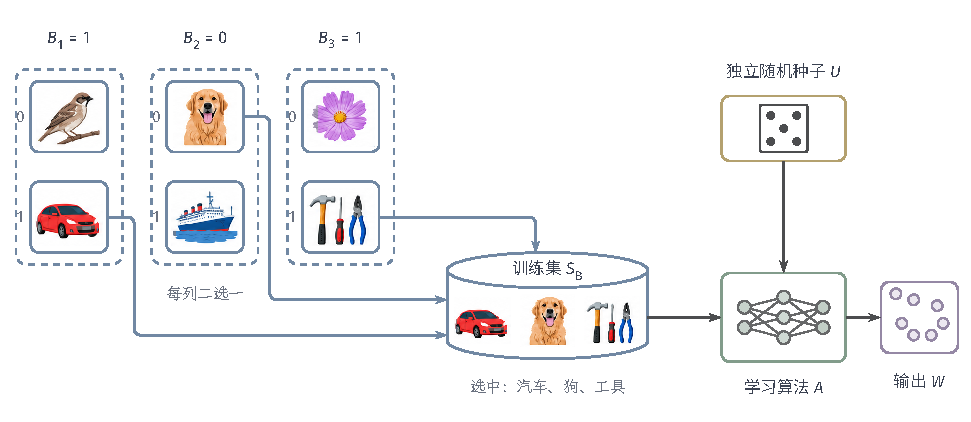
\includegraphics[width=164.600mm]{figures/03-foundations/02-learning-theory/tikz/learning-theory-conditional-information/figure.pdf}
  \caption{条件互信息的抽样构造。每列有两个独立观测，上、下分别编号0、1；选择变量决定哪一个进入训练样本。图中$\bm B=(1,0,1)$，箭头与训练样本中的内容同时标出选中的观测。算法接收选中的三个观测与独立随机种子$U$；条件互信息衡量已知全部六个观测时，输出对选择变量揭示了多少信息。}
 \label{fig:conditional-information}
\end{figure*}

\begin{definition}[算法的条件互信息量]
\label{def:algorithm-cmi}
在上述构造下，算法在分布$\mathcal P$下的条件互信息量定义为
\[
 \kappa_n(A,\mathcal P)=I(W;\bm B\mid\tilde S).
\]
若存在不依赖分布的$\kappa_n$，使所有允许分布满足
$\kappa_n(A,\mathcal P)\leq\kappa_n$且$\kappa_n/n\to0$，
则称算法序列具有在允许分布族上统一的条件互信息稳定性。
\end{definition}

$\bm B$共有$2^n$种取值，所以$0\leq\kappa_n(A,\mathcal P)\leq n\log2$。这个定义排除了连续输出导致的无穷值，但上界与$n$同阶；要让泛化代价趋于零，还需证明算法实际透露的选择信息是$o(n)$。前面的精确样本均值说明这一步并非自动成立：观测取自连续分布时，$2n$个备选值以概率1使不同选择给出不同的和，已知$\tilde S$后由$W$可以反推出全部$\bm B$，于是$\kappa_n=n\log2$，下面定理的上界停留在常数。条件互信息消除了无穷值，却不能为每个泛化良好的算法给出有效的界。

\begin{theorem}[条件互信息与期望风险]
\label{thm:conditional-information-risk}
设$(Z,\mathcal Z)$与$(\mathcal W,\mathcal B_{\mathcal W})$为标准Borel空间，
$\ell:\mathcal W\times Z\to[0,1]$可测，$\mathcal P$为$Z$上的概率分布。
令
$\tilde S=((z_{i,0},z_{i,1}))_{i=1}^n\sim\mathcal P^{2n}$，
令$\bm B=(B_1,\ldots,B_n)$独立于$\tilde S$并均匀分布于$\{0,1\}^n$，
再令算法内部随机数$U$独立于$\tilde S,\bm B$。定义训练样本
$S_{\bm B}=(z_{1,B_1},\ldots,z_{n,B_n})$，并令可测算法
$A:Z^n\times\mathcal U\to\mathcal W$输出$W=A(S_{\bm B},U)$。
此时$S_{\bm B}\sim\mathcal P^n$，且$U$独立于$S_{\bm B}$。定义
\[
\begin{aligned}
 R_{\mathcal P}(w)
 &=\mathbb E_{z\sim\mathcal P}\ell(w,z),\\
 \hat R_{S_{\bm B}}(w)
 &=\frac1n\sum_{i=1}^n\ell(w,z_{i,B_i}),\\
 \kappa_n(A,\mathcal P)
 &=I(W;\bm B\mid\tilde S).
\end{aligned}
\]
则
\[
 \left|\mathbb E[R_{\mathcal P}(W)-\hat R_{S_{\bm B}}(W)]\right|
 \leq\sqrt{\frac{2\kappa_n(A,\mathcal P)}n}.
\]
\end{theorem}
\begin{proof}
用每对中未被选中的观测评价输出，并减去经验风险，记
\[
 g(\tilde S,\bm B,W)=\frac1n\sum_{i=1}^n
 [\ell(W,z_{i,1-B_i})-\ell(W,z_{i,B_i})].
\]
在真实联合分布$P$下，未选观测独立于训练样本和算法内部随机数，所以
$\mathbb E_Pg=\mathbb E[R_{\mathcal P}(W)-\hat R_{S_{\bm B}}(W)]$。
构造参照分布$Q$：保留$(\tilde S,W)$的联合分布，但在给定$\tilde S$后独立、均匀地
重新抽取$\bm B$。于是$D_{\mathrm{KL}}(P\|Q)=\kappa_n(A,\mathcal P)$。

在$Q$下，给定$\tilde S,W$，每一对的损失差随$B_i$以相同概率取正负两个值，
且绝对值不超过1。各项独立，因此
$\log\mathbb E_Q e^{\lambda g}\leq\lambda^2/(2n)$。
将此式用于式~\eqref{eq:information-change-measure}，对正负两个方向分别取最优$\lambda$，
得到结论。
\end{proof}

若在固定分布$\mathcal P$下，平均经验优化误差至多$\rho_n(\mathcal P)$，风险分解给出平均超额风险界$\sqrt{2\kappa_n(A,\mathcal P)/n}+\rho_n(\mathcal P)$。若存在不依赖分布的上界$\kappa_n,\rho_n$，且$\kappa_n/n\to0$、$\rho_n\to0$，定理~\ref{thm:generalization-optimization-learning}便给出PAC学习，充分条件为$\sqrt{2\kappa_n/n}+\rho_n\leq\varepsilon\delta$。条件互信息使用的参照过程与普通互信息不同，常数不能通过简单替换$I(W;S)$得到。它还可以与始终AERM结合，刻画学习算法的存在性。

\begin{theorem}[条件互信息稳定性与可学习性]
\label{thm:conditional-information-learning}
设$(Z,\mathcal Z)$与$(\mathcal W,\mathcal B_{\mathcal W})$为标准Borel空间，
$\mathcal W$非空，$\ell:\mathcal W\times Z\to[0,1]$可测，并允许$Z$上的所有
概率分布。对每个$n$，假定
$s\mapsto\inf_{w\in\mathcal W}n^{-1}\sum_{i=1}^n\ell(w,z_i)$可测；
随机算法均由可测映射$A_n:Z^n\times\mathcal U\to\mathcal W$表示，其内部随机数
$U$与全部观测独立。定义
\[
 R_{\mathcal P}(w)=\mathbb E_{z\sim\mathcal P}\ell(w,z),
 \qquad
 \hat R_S(w)=\frac1n\sum_{i=1}^n\ell(w,z_i).
\]
对每个$\mathcal P$，再令
$\tilde S=((z_{i,0},z_{i,1}))_{i=1}^n\sim\mathcal P^{2n}$，
令$\bm B=(B_1,\ldots,B_n)$独立于$\tilde S,U$并均匀分布于$\{0,1\}^n$，
定义$S_{\bm B}=(z_{1,B_1},\ldots,z_{n,B_n})$；于是
$S_{\bm B}\sim\mathcal P^n$且$U$独立于$S_{\bm B}$。再定义
\[
 \kappa_n(A_n,\mathcal P)
 =I(A_n(S_{\bm B},U);\bm B\mid\tilde S).
\]
则该问题分布无关PAC可学习，也就是存在随机算法$(B_n)$，使任意
$\varepsilon,\delta\in(0,1)$都有不依赖$\mathcal P$的$n_0$，且所有$n\geq n_0$
均满足
\[
 \mathbb P_{S,U}\!\left\{
 R_{\mathcal P}(B_n(S,U))-\inf_{w\in\mathcal W}R_{\mathcal P}(w)
 \leq\varepsilon\right\}\geq1-\delta,
\]
当且仅当存在随机算法$(A_n)$以及不依赖$\mathcal P$的非负序列
$\rho_n\to0$、$\kappa_n/n\to0$，使每份$s\in Z^n$都满足
\[
 \mathbb E_U\hat R_s(A_n(s,U))
 -\inf_{w\in\mathcal W}\hat R_s(w)\leq\rho_n,
\]
并且每个$Z$上的概率分布$\mathcal P$都满足
\[
 \kappa_n(A_n,\mathcal P)\leq\kappa_n.
\]
\end{theorem}
\begin{proof}
充分性由定理~\ref{thm:conditional-information-risk}与
定理~\ref{thm:generalization-optimization-learning}给出。
为证必要性，使用一般学习基本定理证明中的构造：从$n$个位置中有放回地随机抽取
$k=\lfloor\sqrt n\rfloor$个位置，再调用已有学习算法。该构造已经保证始终AERM。

记抽样索引为$J=(J_1,\ldots,J_k)$，原学习算法的内部随机数为$U_0$。
在给定$\tilde S,J,U_0$时，新算法的输出仅由被访问位置的选择变量
$(B_{J_1},\ldots,B_{J_k})$决定。每个选择变量至多包含$\log2$的信息量，故
\begin{align*}
 I(W;\bm B\mid\tilde S)
 &\leq I(W,J,U_0;\bm B\mid\tilde S)\\
 &=I(W;\bm B\mid\tilde S,J,U_0)
 \leq k\log2.
\end{align*}
等式使用$J,U_0$与$\tilde S,\bm B$独立；最后一步使用互信息不超过决定输出的
离散选择变量的熵。因此可取$\kappa_n=k\log2$，并有$\kappa_n/n\to0$。
\end{proof}

这里的必要性同样允许重新构造算法，并不要求每个成功算法本身的条件互信息都小。也不能把条件互信息换成普通互信息，因为后者仍会记录连续观测的无限精度。

\subsection{稳定性的关系与边界}
\label{sec:stability-comparison}

现在可以在同一个风险目标下比较这些条件。留一法、均匀稳定性和平均稳定性都比较损失，但分别改变了训练样本的扰动方式、评价观测和取平均的方法；有的先取绝对值，有的保留正负号。参数稳定性把直接比较的对象改为参数距离，需要借助损失的变化率转换回风险。信息方法则比较真实联合分布与独立参照分布，不需要给参数定义距离。这些条件得到的上界形式不同，但都要与经验优化误差结合，才能判断学习是否成功。

回到第~\ref{sec:real-valued-classes}节的反例，可以看清稳定性路线为什么能走到一致收敛走不到的地方。始终输出$w_0$的算法，在任何相邻样本上输出都相同，均匀稳定性常数为零；$w_0$的经验风险恒为0，等于经验最优值，经验优化误差也为零。两项代入风险分解，立即得到学习保证。一致收敛在这个例子中失败，是因为它要求估计准确那些有限集决策的风险；稳定性只检查算法实际选择的$w_0$，那些决策是否难以估计与它无关。

固定替换这一扰动方式，均匀损失界蕴含平均损失界；再加上统一的Lipschitz条件，均匀或平均的参数界可以分别转换成对应的损失界。删除会改变样本量，删除条件与替换条件不能直接等同。参数距离也必须先经损失条件转换，不能跳过这一步直接当作风险代价。

互信息稳定性与均匀损失稳定性之间没有一般的强弱关系。样本均值算法有趋于零的均匀稳定性，但它的普通互信息为无穷。反方向可取$z_i\in\{0,1\}$的二值观测：算法只在样本全为1时输出$W=1$，否则输出0，损失为$\ell(w,z)=w$。输出只有两种可能，故$I(W;S)\leq\log2$；但把全1样本中的任意一项替换为0，输出就从1变为0，损失改变1，均匀稳定性常数无法随$n$下降。可见小的信息代价只控制平均依赖，不控制每一对相邻样本。

这个二值例子也区分了信息依赖与学习效果。当分布只产生1时，训练样本必为全1，算法输出1，损失也恒为1；决策0的损失却恒为0。此时输出在该分布下是常量，互信息为零，但在所有可能的相邻样本之间，它仍不满足趋于零的均匀稳定性。无论如何，小互信息没有弥补经验优化的失败，因此不能单独推出低风险。

定理~\ref{thm:general-stability-characterization}、定理~\ref{thm:average-stability-characterization}和定理~\ref{thm:conditional-information-learning}分别用均匀稳定、平均稳定和条件互信息稳定的始终AERM算法刻画可学习性。这些都是算法存在性的结论；留一法稳定性、参数稳定性和普通互信息则提供了验证具体算法的充分途径，不能转化为每个成功算法都必须满足的必要性质。表~\ref{tab:stability-object-comparison}汇总了各条件直接控制的对象，图~\ref{fig:learning-risk-routes}比较它们与一致收敛共同的证明目标。

\begin{table*}[htbp]
 \centering
 \footnotesize
 \begin{tabularx}{\linewidth}{@{}l l X X X@{}}
  \toprule
  \textbf{条件} & \textbf{训练样本扰动} & \textbf{直接比较对象} &
  \textbf{平均或最坏情形} & \textbf{进入学习保证还需什么} \\
  \midrule
  留一法稳定性 & 删除一项 & 被删观测上的损失 &
  对样本和位置平均 & 经验最优性；注意$n$与$n-1$的算法错位 \\
  均匀稳定性 & 替换一项 & 任意测试观测上的损失差 &
  对相邻样本和测试观测取最坏情形 & 经验最优性；高概率界还需损失有界 \\
  平均稳定性 & 替换一项 & 被替换出的$z_i$上的有符号损失差 &
  对样本、位置、替换值和随机性平均 & 允许分布族上的统一速率与经验最优性 \\
  参数稳定性 & 替换一项 & 共享随机数下的参数距离 &
  可取最坏情形或平均 & 损失关于参数的Lipschitz性或非负光滑损失的自界关系，以及经验最优性；光滑分支还需统一控制均方根距离与损失规模 \\
  互信息稳定性 & 不显式构造邻样本 & $I(W;S)$ &
  对训练样本和算法随机性定义的分布量 & 有界或次高斯损失，以及经验最优性 \\
  条件互信息稳定性 & 双样本逐位选择 & 已知双样本时输出揭示的选择信息 &
  对双样本、选择位和随机性定义的分布量 & 有界损失；可学习性刻画还需始终AERM \\
  \bottomrule
 \end{tabularx}
 \caption{各类稳定性及算法依赖条件的对象与保证接口。表中条件之间不存在未注明的一般强弱关系。}
 \label{tab:stability-object-comparison}
\end{table*}

\begin{figure*}[htbp]
  \centering
  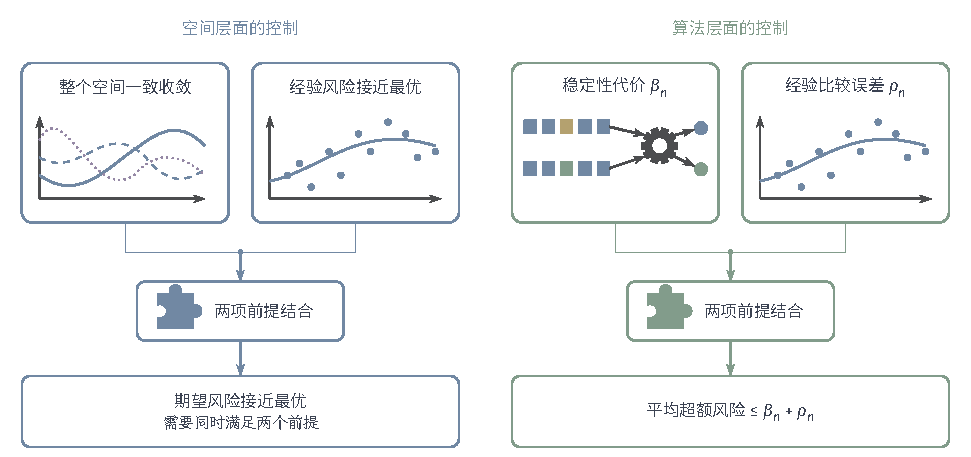
\includegraphics[width=164.600mm]{figures/03-foundations/02-learning-theory/tikz/learning-theory-risk-routes/figure.pdf}
  \caption{期望风险的两条分析路线。左侧同时控制整个决策空间，右侧控制算法输出的期望
 泛化差；两条路线都要结合经验最优性。右侧用$\beta_n$泛指所选稳定性定理提供的代价项。}
 \label{fig:learning-risk-routes}
\end{figure*}

\FloatBarrier
\section{凸学习问题}
\label{sec:regularized-learning}
\label{sec:convex-learning-problem}

第~\ref{sec:algorithmic-stability}节把学习保证分成两项：算法不能过度依赖个别训练观测，同时要在训练样本上取得接近最优的平均损失。基本定理证明了可学习时存在这样的算法，但它构造的算法（随机抽取$\sqrt n$项再调用某个已知学习算法）只用于证明存在性。实际使用的是正则化最小化和梯度下降一类算法，我们需要对它们逐一算出稳定性代价$\beta_n$和经验优化误差$\rho_n$。

这一步在零一损失下很难完成。零一损失关于参数是分段常数：参数的微小移动可能让损失从0跳到1，所以参数距离控制不住损失差；它的梯度几乎处处为零，梯度方法也得不到改进方向。凸学习问题提供了恰好需要的结构。凸性使局部的下降方向指向全局最优，经验优化误差可以随迭代算出；在凸性之上，强凸性限制最优解随样本的移动，光滑性保证一次梯度更新不扩大两条轨迹的距离；Lipschitz性再把参数距离换算成损失差。

本节比较两种做法：在经验目标中加入正则项后求最优解，或者运行有限步随机梯度下降。两者都先比较相邻样本上的训练结果，得到期望泛化差的上界，再回到原问题，检查输出的经验风险比最低经验风险高出多少。正则化需要另外估计改变目标带来的代价，SGD需要估计尚未完成优化的误差，这两种代价都不能被稳定性保证替代。弱凸性和PL条件留到非凸问题中讨论（最优化的基本概念可参考\BookVolumeRef{vol:mathematical-preliminaries-upper}{卷1《数学准备：计算、分析与几何》}）。

\subsection{凸性与损失函数}

我们先看怎样把一个具体任务写成凸学习问题。对线性分类器，预测由分数$\bm w^\top\bm x$的符号决定。真实标签为$+1$时，分数从$-2$提高到$-0.1$，零一损失仍为1；它在判定阈值处跳变，其余位置的导数为零，不能为梯度更新提供改进方向。因此训练时常用合页损失$\max\{0,1-y\bm w^\top\bm x\}$或逻辑损失$\log(1+e^{-y\bm w^\top\bm x})$。两者关于线性参数$\bm w$都是凸函数。合页损失在上述例子中从3降到1.1，分数达到1后才降为零；它还要求正确分类具有一定间隔。逻辑损失可微，而合页损失在拐点处不可微，所以二者都能用于凸正则化的分析，却不能不加区分地套用后面的光滑SGD定理。

改用损失也改变了训练要最小化的风险。为了把替代风险的改进联系到分类错误率，还需要\term{分类校准}（classification calibration）：它要求在不限制预测函数表达能力时，替代风险趋于最优能够带来零一风险趋于贝叶斯风险。凸性解决的是怎样优化替代目标，校准解决的是这个目标是否与分类评价相容。

校准考察固定输入时的标签选择。记$\eta(x)=\mathbb P(y=1\mid x)$，按这个条件分布对替代损失取期望，得到给定输入下的条件替代风险。$\eta(x)>1/2$时最优分数应取正号，$\eta(x)<1/2$时应取负号。例如正标签概率为0.7时，预测正类的错误率为0.3，预测负类为0.7，因此校准要求替代损失的最优分数也偏向正号。凸性帮助求解，校准则把不受限函数空间中的替代最优风险与贝叶斯风险联系起来。在受限的线性函数类中，替代最优解不一定也是零一最优解，还要检查线性类的近似能力。这里的分类校准不同于第~\ref{sec:reliability-output-evaluation}节的概率校准：后者比较预测概率与事件发生的频率，二者之间没有一般的相互蕴含关系。

这个例子提示了凸学习的两个要求：任意两个允许的决策之间作线性插值，仍应得到允许的决策；插值后的损失不应超过两端损失的对应加权平均。本节用实赋范线性空间$(V,\|\cdot\|)$描述决策，取$\mathcal W\subseteq V$。凸性由线性结构定义；Lipschitz常数和强凸常数还依赖所选范数，比较这些常数时必须使用同一范数。

\begin{definition}[凸学习问题]
\label{def:convex-learning-problem}
若$\mathcal W$是凸集，并且对每个$z\in Z$，函数$w\mapsto\ell(w,z)$为凸函数，则称
该一般学习问题为凸学习问题。也就是说，对任意$u,v\in\mathcal W$、$t\in[0,1]$和$z\in Z$，有
\[
 \ell(tu+(1-t)v,z)\leq t\ell(u,z)+(1-t)\ell(v,z).
\]
\end{definition}

前面两种替代损失都可以按定义核对。合页损失是两个关于$\bm w$的仿射函数$0$与$1-y\bm w^\top\bm x$的逐点最大值，而凸函数的逐点最大值仍凸；逻辑损失是$s\mapsto\log(1+e^{-s})$与线性函数$s=y\bm w^\top\bm x$的复合，前者的二阶导数$e^{-s}/(1+e^{-s})^2>0$，复合线性映射保持凸性。对固定样本，各条损失的平均仍是凸函数，因此经验风险也是凸的。不过，凸性并没有限制参数移动一点时损失能够变化多少。后面先估计相邻样本上两个解的距离，再用这一距离估计损失差，所以还需要第~\ref{sec:parameter-stability}节式~\eqref{eq:parameter-loss-lipschitz}用过的Lipschitz条件，这里把欧氏范数换成决策空间上的一般范数。例如常数$L=2$时，参数移动距离0.01，在同一个观测上的损失变化至多为0.02。这里比较的是损失值，而SGD分析中的光滑性比较的是梯度；两项条件不能混为一谈。

\begin{definition}[Lipschitz损失]
\label{def:lipschitz-loss}
若对任意$w,w'$与$z$都满足
\begin{equation}
 |\ell(w,z)-\ell(w',z)|\leq L\|w-w'\|,
 \label{eq:lipschitz-loss}
\end{equation}
则称损失关于该范数是$L$-Lipschitz的。
\end{definition}

凸性针对训练时真正优化的变量。损失关于预测分数凸，并不保证把分数写成神经网络后，它关于网络参数仍然凸。以下两小节都在已经确认的凸决策空间和凸损失上工作：正则化比较两个经验目标的最优解，SGD比较有限次更新产生的输出。选择哪种分析，取决于实际运行的算法，而不是损失函数的名称。

除稳定性外，欧氏空间中范数受限的线性预测也可以继续使用一致收敛路线：$\|\bm w\|_2\leq B$且$\|\bm x\|_2\leq r$时，式~\eqref{eq:linear-rademacher-bound}给出得分函数类的Rademacher复杂度上界$Br/\sqrt n$；若损失关于得分为$L$-Lipschitz，收缩引理给出损失类复杂度上界$LBr/\sqrt n$。收缩引理说的是：把函数类的每个函数复合上同一个$L$-Lipschitz的标量函数，Rademacher复杂度至多乘以$L$。这里Lipschitz性又一次承担“把得分的差异换算成损失的差异”的作用。配合有界或合适的尾部条件后，可用它估计风险。下面的稳定性分析是一种算法层面的替代方法，并不是说凸问题只能用稳定性分析。

\subsection{凸学习问题的正则化}

当经验目标在一片区域内很平坦时，替换一条训练观测就可能使最优解从一端移到另一端。以绝对损失$\ell(w,z)=|w-z|$为例，取两条观测$z_1=0$、$z_2=1$，经验风险在整个区间$[0,1]$上都等于$1/2$，每个点都是经验最优解。若算法在并列者中取最左端，输出为0；把$z_1$换成$1$后，最优解只剩$w=1$。两个目标只差一项，输出却移动了整个区间。我们希望加入一个确定的惩罚项，使偏离最优位置会产生足够大的目标增量，从而限制这种移动。取$\lambda>0$，用$\Omega(w)$表示惩罚，定义正则化算法
\begin{equation}
 A(S)\in\argmin_{w\in\mathcal W}
 \left\{\hat R_S(w)+\lambda\Omega(w)\right\}.
 \label{eq:regularized-erm}
\end{equation}
这里$\lambda$决定经验损失与惩罚的相对权重；仅仅添加惩罚并不保证稳定。接下来选择能使整个目标强凸的惩罚。若存在$\mu>0$，使目标函数$F$满足
\begin{equation}
 F(tu+(1-t)v)\leq tF(u)+(1-t)F(v)
 -\frac\mu2t(1-t)\|u-v\|^2
 \label{eq:strong-convexity}
\end{equation}
对所有可行$u,v$及$t\in[0,1]$成立，则称$F$为$\mu$-强凸。与凸性相比，右端多减去一个与$\|u-v\|^2$成正比的量，要求函数在两点之间不能过于平坦。例如$F(w)=\mu w^2/2$恰好取等号，而常数函数是凸的却不强凸。若最小点$w_*$存在，取$u=w$、$v=w_*$，左侧不小于最小值$F(w_*)$，整理得$t(F(w)-F(w_*))\geq\frac\mu2t(1-t)\|w-w_*\|^2$；两边除以$t$再令$t\to0$，得到二次增长
\[
 F(w)-F(w_*)\geq\frac\mu2\|w-w_*\|^2.
\]
它说明：离最小点越远，目标值必定高出越多。这比较的是任意决策与最小点，而不是任意两个决策；不同决策仍可能有相同目标值。

这一最小点附近的二次下界正是稳定性证明需要的工具。设两个相邻样本的最优解为$w$和$w'$。先用第一个目标比较$w'$与它的最小点$w$，再用第二个目标比较$w$与它的最小点$w'$；两个比较都给出距离平方的下界。将它们相加后，样本中相同的$n-1$项及相同正则项抵消，只剩被替换观测的贡献。因而一次样本替换能够引起多大参数移动，可以由这一个观测的损失变化来限制。

这一作用在均值估计中可以显式算出。对$z_i\in[0,1]$，最小化
\[
 \frac1{2n}\sum_{i=1}^n(w-z_i)^2+\frac\lambda2w^2
\]
可得最优解$\hat w=\bar z/(1+\lambda)$，替换一项后至多移动$1/[n(1+\lambda)]$。增大$\lambda$减小了移动，但也使输出偏向零：若总体均值为$m$，输出的期望为$m/(1+\lambda)$，偏离$m$的量为$\lambda m/(1+\lambda)$。稳定性的收益与偏差的代价都由同一个$\lambda$决定，这是后面风险界中两项此消彼长的雏形。下面先证明一般稳定性界，再计算这种目标改变可能带来的风险代价。定理要求损失为$L$-Lipschitz、惩罚$\Omega$为1-强凸，因此整个正则目标为$\lambda$-强凸。

\begin{theorem}[强凸正则化的稳定性]
\label{thm:regularized-erm-stability}
设$(Z,\mathcal Z)$为可测观测空间，$\mathcal W$是实赋范线性空间
$(V,\|\cdot\|)$中的非空凸Borel集，$\ell:\mathcal W\times Z\to\mathbb R$可测。
对每个$z\in Z$，函数$\ell(\cdot,z)$在$\mathcal W$上凸，并且对任意
$u,v\in\mathcal W$都有
\[
 |\ell(u,z)-\ell(v,z)|\leq L\|u-v\|.
\]
设$\Omega:\mathcal W\to\mathbb R$可测，且对任意$u,v\in\mathcal W$和
$t\in[0,1]$都有
\[
 \Omega(tu+(1-t)v)
 \leq t\Omega(u)+(1-t)\Omega(v)-\frac12t(1-t)\|u-v\|^2.
\]
固定$n\geq1$与$\lambda>0$。对任意$Z$上的概率分布$\mathcal P$，
训练样本满足$S\sim\mathcal P^n$；对每份$s=(z_1,\ldots,z_n)\in Z^n$，定义
\[
 A(s)\in\argmin_{w\in\mathcal W}
 \left\{\frac1n\sum_{i=1}^n\ell(w,z_i)+\lambda\Omega(w)\right\},
\]
并假定该最小解存在且$A$可测。目标函数的强凸性使最小解唯一；对任意只相差一个
观测的$s,s'\in Z^n$及任意$z\in Z$，算法满足
\[
 |\ell(A(s),z)-\ell(A(s'),z)|\leq\beta_n,
\]
并且其稳定性常数满足
\begin{equation}
 \beta_n\leq\frac{2L^2}{\lambda n}
 \label{eq:regularized-stability-bound}
\end{equation}
\end{theorem}

\begin{proof}
记相邻样本的最优解为$w=A(S)$和$w'=A(S')$，相应正则目标为$F_S$和$F_{S'}$。两个目标不能直接比较最小值，因为它们使用了不同观测。我们分别在每个目标内比较这两个参数：在$F_S$中，$w$是最小点；在$F_{S'}$中，$w'$是最小点。由$\lambda$-强凸性，得到
\begin{equation*}
 F_S(w')-F_S(w)\geq\frac\lambda2\|w-w'\|^2,
 \quad
 F_{S'}(w)-F_{S'}(w')\geq\frac\lambda2\|w-w'\|^2.
\end{equation*}
将两个不等式相加。设$S$与$S'$只在第$i$项不同，分别为$z_i$与$z_i'$。左侧重新按观测整理后，相同的$n-1$个损失项和相同的正则项全部抵消，只剩
\[
 \frac1n\Bigl[\ell(w',z_i)-\ell(w,z_i)+\ell(w,z_i')-\ell(w',z_i')\Bigr]
 \geq\lambda\|w-w'\|^2.
\]
方括号内两组差各由Lipschitz性控制为$L\|w-w'\|$，便得到$\lambda\|w-w'\|^2\leq2L\|w-w'\|/n$。左侧随距离平方增长，右侧只随距离线性增长，所以距离不可能太大。若两解相同，距离界直接成立；否则除以$\|w-w'\|$，得到$\|w-w'\|\leq2L/(\lambda n)$。最后在任意测试观测$z$上再用一次Lipschitz条件：
\[
 |\ell(w,z)-\ell(w',z)|
 \leq L\|w-w'\|
 \leq\frac{2L^2}{\lambda n},
\]
即得到所述均匀稳定性上界。
\end{proof}

到这里，我们只控制了相邻样本之间的输出差：参数距离至多$2L/(\lambda n)$，再用Lipschitz条件得到损失差至多$2L^2/(\lambda n)$。在所需可积性成立时，均匀稳定性定理便给出同样大小的期望泛化差上界。以$L_2$正则的逻辑回归为例：设$\|\bm x\|_2\leq r$，逻辑损失$\log(1+e^{-y\bm w^\top\bm x})$关于$\bm w$的梯度为$-y\bm x/(1+e^{y\bm w^\top\bm x})$，范数不超过$r$，所以它关于参数是$r$-Lipschitz的凸损失；取$\Omega(\bm w)=\|\bm w\|_2^2/2$，稳定性常数至多$2r^2/(\lambda n)$。若$r=1$、$\lambda=0.1$、$n=1000$（教学取值），上界为$0.02$。这还没有说明输出接近原问题的最优风险。

平方损失应用这个定理时需特别核对区域。岭回归使用$\Omega(w)=\|w\|_2^2/2$。在欧氏或一般Hilbert范数下，展开$\|tu+(1-t)v\|^2$可知它使强凸不等式恰好取等号，所以它是1-强凸的；换成其他范数的平方，这一性质未必成立。另一方面，平方损失在无界参数上没有全局Lipschitz常数；限制输入、标签和参数后，才能通过残差的上界得到这里所需的有限$L$。

接着比较原来的风险目标。算法最小化的是$\hat R_S(w)+\lambda\Omega(w)$，而我们评价的仍是$R_{\mathcal P}(w)$，不是加了惩罚的风险。对任何事先固定的比较决策$w$，正则目标的最优性保证$\hat R_S(A(S))\leq\hat R_S(w)+\lambda\Omega(w)$，其中用到了$\Omega\geq0$。对样本平均后，右侧的经验风险变成$R_{\mathcal P}(w)$；左侧再加上刚才的期望泛化差上界，就得到下一个定理。这样，正则化的作用与代价分别出现在两项中。

\begin{theorem}[正则化学习的期望风险保证]
\label{thm:regularized-learning-risk}
设$(Z,\mathcal Z)$为可测观测空间，$\mathcal W$是实赋范线性空间
$(V,\|\cdot\|)$中的非空凸Borel集，$\ell:\mathcal W\times Z\to\mathbb R$可测。
对每个$z\in Z$，函数$\ell(\cdot,z)$在$\mathcal W$上凸，并且对任意
$u,v\in\mathcal W$都有
\[
 |\ell(u,z)-\ell(v,z)|\leq L\|u-v\|.
\]
设$\Omega:\mathcal W\to[0,\infty)$可测，且对任意$u,v\in\mathcal W$和
$t\in[0,1]$都有
\[
 \Omega(tu+(1-t)v)
 \leq t\Omega(u)+(1-t)\Omega(v)-\frac12t(1-t)\|u-v\|^2.
\]
固定$n\geq1$与$\lambda>0$。令$S=(z_1,\ldots,z_n)\sim\mathcal P^n$，其中
$\mathcal P$为$Z$上的概率分布，并定义可测算法
\[
 A(S)=\argmin_{v\in\mathcal W}
 \left\{\frac1n\sum_{i=1}^n\ell(v,z_i)+\lambda\Omega(v)\right\}.
\]
再令$z\sim\mathcal P$独立于$S$，并定义
\[
 R_{\mathcal P}(w)=\mathbb E_{z\sim\mathcal P}\ell(w,z),
 \qquad
 \hat R_S(w)=\frac1n\sum_{i=1}^n\ell(w,z_i).
\]
假定该最小解存在；独立测试损失$\ell(A(S),z)$、训练损失
$\ell(A(S),z_i)$以及每个固定$w\in\mathcal W$的$\ell(w,z)$均可积。
则对任意固定$w\in\mathcal W$，
\begin{equation}
 \mathbb E_S R_{\mathcal P}(A(S))-R_{\mathcal P}(w)
 \leq\frac{2L^2}{\lambda n}+\lambda\Omega(w).
 \label{eq:regularization-excess-risk}
\end{equation}
若$\mathcal W=\{w:\|w\|\leq B\}$为Hilbert空间中以原点为中心、半径为$B>0$的闭球，$\Omega(w)=\|w\|^2/2$，
且$L>0$，取$\lambda=2L/(B\sqrt n)$可得
\[
 \mathbb E_S R_{\mathcal P}(A(S))-\inf_{w\in\mathcal W}R_{\mathcal P}(w)
 \leq\frac{2LB}{\sqrt n}.
\]
\end{theorem}
\begin{proof}
正则化目标的最优性给出
\[
 \hat R_S(A(S))+\lambda\Omega(A(S))
 \leq\hat R_S(w)+\lambda\Omega(w).
\]
由于$\Omega(A(S))\geq0$，去掉左侧的正则项后仍有$\hat R_S(A(S))\leq\hat R_S(w)+\lambda\Omega(w)$。比较决策$w$在抽样前固定，所以$\mathbb E_S\hat R_S(w)=R_{\mathcal P}(w)$；算法输出则依赖样本，必须借助稳定性才能把它的经验风险换成期望风险，两者的期望差至多为$2L^2/(\lambda n)$。两步合并得到第一式。

在半径$B$的闭球内，$\Omega(w)=\|w\|^2/2\leq B^2/2$。代入所给$\lambda$，两项上界各不超过$LB/\sqrt n$，且对每个比较决策$w$都相同。对$w$取下确界，即得第二式，不要求存在取到下确界的决策。
\end{proof}

式~\eqref{eq:regularization-excess-risk}由两项组成：$2L^2/(\lambda n)$来自样本替换的稳定性，$\lambda\Omega(w)$来自改用正则目标后与原比较决策的差距。这正是正则化与稳定性的联系：$\lambda$越大，目标的强凸性越强，解越不随单条观测移动；但目标也越偏离原来的经验风险。增大$\lambda$会减小前一上界、增大后一上界，并不说明实际风险一定随之上升或下降。在半径为$B$的球内，$\Omega(w)\leq B^2/2$对所有比较决策成立，上界变为$2L^2/(\lambda n)+\lambda B^2/2$；令两项相等解出$\lambda=2L/(B\sqrt n)$，即定理中的取值，此时两项都等于$LB/\sqrt n$。样本越多，单条观测的影响本来就越小，所需的正则化也就越弱，$\lambda$按$1/\sqrt n$减小。由此先得到平均超额风险界，再利用超额风险非负和Markov不等式得到充分样本量$n\geq(2LB/(\varepsilon\delta))^2$，未声称这一置信度依赖最优。

这个结论不显含参数维数，但依赖于半径$B$和损失变化率$L$受到统一控制。它不与二分类的不可学习性结果矛盾：一般的零一分类损失既不是这里的凸损失，也不满足所需的参数Lipschitz条件。以上还假定正则目标被精确最小化；若只运行有限次优化，实际求解误差需要另外计入。下一小节直接研究这种有限次训练。

\subsection{凸学习问题的随机梯度下降}
\label{sec:sgd-stability}

上一小节把正则目标的精确最优解作为算法输出。实际训练中，我们常按步更新参数，并在有限次更新后停止。本小节直接分析随机梯度下降（stochastic gradient descent, SGD）：每次从固定训练样本中随机选一条观测，用它的损失梯度更新参数。以$\ell(w,z)=(w-z)^2/2$为例，从$w=0.5$出发、步长为0.1，抽到$z=0$时更新到0.45，抽到$z=1$时更新到0.55。这个例子说明随机索引怎样影响轨迹，并不作为全局有界梯度的例子。

固定一份$n$项样本，令各$i_t$独立均匀地取自$\{1,\ldots,n\}$，从确定的初值开始迭代：
\begin{equation}
 \bm w^{(t+1)}=\bm w^{(t)}-\eta_t\nabla\ell(\bm w^{(t)},z_{i_t}),
 \qquad t=0,\ldots,T-1.
 \label{eq:sgd-update}
\end{equation}
这里每步都从同一份训练样本中抽取索引，可以重复访问某条观测，并不是每步从总体获得新数据。为分析样本替换的影响，在两份相邻样本上使用相同初值和相同索引序列；在第一次访问被替换位置之前，两条轨迹完全相同。

之后的距离怎样变化，需要分别控制两个因素。损失为$L$-Lipschitz且可微，保证梯度范数不超过$L$：沿梯度方向移动距离$r$，损失约变化$r\|\nabla\ell\|_2$，而Lipschitz性要求它不超过$Lr$。因此一次不同观测带来的更新差有限。损失为$M$-光滑，指$\|\nabla\ell(\bm u,z)-\nabla\ell(\bm v,z)\|_2\leq M\|\bm u-\bm v\|_2$：参数相近时，梯度也不会相差太多。再结合凸性和步长$\eta_t\leq2/M$，同一条观测上的更新不会扩大已有的参数距离。下面的定理据此先计算稳定性，暂不保证经验风险已经很小。

\begin{theorem}[凸光滑SGD的稳定性]
\label{thm:convex-sgd-stability}
设$(Z,\mathcal Z)$为可测观测空间，
$\ell:\mathbb R^d\times Z\to\mathbb R$可测。对每个$z\in Z$，
$\ell(\cdot,z)$可微、凸、$L$-Lipschitz且$M$-光滑，其中$M>0$，即
\[
\begin{aligned}
 |\ell(\bm u,z)-\ell(\bm v,z)|
 &\leq L\|\bm u-\bm v\|_2,\\
 \|\nabla\ell(\bm u,z)-\nabla\ell(\bm v,z)\|_2
 &\leq M\|\bm u-\bm v\|_2,
 \qquad \bm u,\bm v\in\mathbb R^d.
\end{aligned}
\]
固定$n,T\geq1$、确定初值$\bm w^{(0)}\in\mathbb R^d$以及步长
$0\leq\eta_t\leq2/M$。任取$Z$上的概率分布$\mathcal P$并令
$S=(z_1,\ldots,z_n)\sim\mathcal P^n$。算法内部随机数
$U=(i_0,\ldots,i_{T-1})$独立于$S$，并由独立且均匀分布于
$\{1,\ldots,n\}$的索引组成；算法更新
\[
 \bm w^{(t+1)}
 =\bm w^{(t)}-\eta_t\nabla\ell(\bm w^{(t)},z_{i_t}),
 \qquad t=0,\ldots,T-1.
\]
令$A_{n,T}(S,U)=\bm w^{(T)}$。比较相邻样本时，两次运行使用相同的初值和$U$。
则任意只相差一个观测的$S,S'\in Z^n$及任意$z\in Z$都满足
\[
 \left|\mathbb E_U\ell(A_{n,T}(S,U),z)
 -\mathbb E_U\ell(A_{n,T}(S',U),z)\right|\leq\beta_n,
\]
其中
\[
 \beta_n\leq\frac{2L^2}{n}\sum_{t=0}^{T-1}\eta_t.
\]
\end{theorem}
\begin{proof}
在相邻样本上共享同一索引序列，将一次更新分成“抽到共同观测”和“抽到替换位置”两种情况。先看共同观测。凸且$M$-光滑的损失具有以下梯度性质：
\[
 \langle\nabla\ell(\bm u,z)-\nabla\ell(\bm v,z),\bm u-\bm v\rangle
 \geq\frac1M\|\nabla\ell(\bm u,z)-\nabla\ell(\bm v,z)\|_2^2.
\]
记梯度差$\bm\Delta=\nabla\ell(\bm u,z)-\nabla\ell(\bm v,z)$，展开同一观测更新后的距离平方，并代入上式：
\[
 \|(\bm u-\eta_t\nabla\ell(\bm u,z))-(\bm v-\eta_t\nabla\ell(\bm v,z))\|_2^2
 \leq\|\bm u-\bm v\|_2^2-\eta_t\Bigl(\frac2M-\eta_t\Bigr)\|\bm\Delta\|_2^2.
\]
当$0\leq\eta_t\leq2/M$时最后一项非正，所以同一损失的梯度映射不扩大距离。这控制了共同观测上的更新。抽中替换位置时，可先比较使用同一观测更新的结果，再计入把该观测换掉产生的额外变化；两个梯度的范数都至多为$L$，这部分变化至多为$2\eta_tL$。

令$d_t=\mathbb E\|\bm w^{(t)}-\bm w'^{(t)}\|_2$，期望只对共同索引序列取。每步以$1/n$的概率访问替换位置，因此$d_{t+1}\leq d_t+2\eta_tL/n$。从$d_0=0$累加，再用Lipschitz性转换为损失差，得到
\begin{equation}
 d_T\leq\frac{2L}{n}\sum_{t=0}^{T-1}\eta_t,
 \qquad
 \beta_n\leq\frac{2L^2}{n}\sum_{t=0}^{T-1}\eta_t.
 \label{eq:convex-sgd-stability}
\end{equation}
\end{proof}

这个证明沿着“共享索引—区分是否访问替换位置—累加参数距离—换成损失差”推进。未访问替换位置时，更新不扩大已有距离；访问时至多增加$2L\eta_t$，而发生概率为$1/n$。所以稳定性上界取决于步长之和，而不是单独取决于迭代次数。例如$L=1$、$n=1000$、固定步长$\eta=0.01$时，训练$T=n$步的上界为$2\times0.01\times1000/1000=0.02$；训练$10n$步则为$0.2$。这里的数值只是代入公式的教学示例，说明上界随总步长线性增长。结论对每对相邻样本成立，只对共享索引序列平均，因而可以通过第~\ref{sec:algorithmic-stability}节的均匀稳定性结论估计期望泛化差。

式~\eqref{eq:convex-sgd-stability}的上界随总步长增大。另一方面，过早停止可能留下较大的经验优化误差。因此，它只能说明延长训练可能增加这一泛化上界，不能单独确定最佳停止时刻。接下来先看加强凸性后能否改善稳定性，再回到普通凸条件，把优化误差加入完整的学习保证。相关的SGD稳定性分析见Hardt、Recht与Singer\scite{hardt2016sgd}。

如果每条观测的损失在可行区域内都强凸，同一观测上的更新还能缩小已有距离，而不仅仅是不扩大它。于是早期替换造成的影响会随后续更新衰减，新产生的影响不再简单累加。下一个定理研究这一更强条件下的投影SGD：每次更新后投影回闭凸集，以保证参数留在条件成立的区域内。强凸性和梯度有界都只在该区域要求；非平凡函数不可能在整个欧氏空间上既全局强凸又具有全局有界梯度。

\begin{theorem}[强凸投影SGD的稳定性]
\label{thm:strongly-convex-sgd-stability}
设$(Z,\mathcal Z)$为可测观测空间，
$\mathcal W\subseteq\mathbb R^d$是非空闭凸集，
并令$\mathcal O\subseteq\mathbb R^d$为包含$\mathcal W$的开集。
设$\ell:\mathcal O\times Z\to\mathbb R$可测，且每个$\ell(\cdot,z)$在
$\mathcal O$上二阶连续可微。对任意$\bm w\in\mathcal W,z\in Z$，假定
\[
 \mu\bm I\preceq\nabla^2\ell(\bm w,z)\preceq M\bm I,
 \qquad \|\nabla\ell(\bm w,z)\|_2\leq L,
\]
其中$0<\mu\leq M$。固定$n,T\geq1$、初值$\bm w^{(0)}\in\mathcal W$及步长
$0<\eta\leq1/M$。任取$Z$上的概率分布$\mathcal P$并令
$S=(z_1,\ldots,z_n)\sim\mathcal P^n$。算法内部随机数
$U=(i_0,\ldots,i_{T-1})$独立于$S$，并由独立且均匀分布于
$\{1,\ldots,n\}$的索引组成；算法更新
\[
 \bm w^{(t+1)}
 =\Pi_{\mathcal W}\!\left(
 \bm w^{(t)}-\eta\nabla\ell(\bm w^{(t)},z_{i_t})\right),
 \qquad t=0,\ldots,T-1.
\]
令$A_{n,T}(S,U)=\bm w^{(T)}$。比较相邻样本时，两次运行共享初值和$U$。
则任意只相差一个观测的$S,S'\in Z^n$及任意$z\in Z$都满足
\[
 \left|\mathbb E_U\ell(A_{n,T}(S,U),z)
 -\mathbb E_U\ell(A_{n,T}(S',U),z)\right|\leq\beta_{n,T},
\]
其中
\[
 \beta_{n,T}\leq\frac{2L^2}{\mu n}
           \bigl(1-(1-\mu\eta)^T\bigr)
 \leq\frac{2L^2}{\mu n}.
\]
\end{theorem}
\begin{proof}
沿两参数之间的线段对Hessian积分，梯度更新的差等于
$(\bm I-\eta\bm H)(\bm u-\bm v)$，其中$\bm H$的特征值位于$[\mu,M]$。
$\bm I-\eta\bm H$的特征值位于$[1-\eta M,1-\eta\mu]$；由$\eta\leq1/M$，它们都在$[0,1-\mu\eta]$内，
所以同一观测的更新将距离至多乘以$1-\mu\eta$。投影不扩大距离。
令$D_t=\mathbb E_U\|\bm w^{(t)}-\bm w'^{(t)}\|_2$，其中两条轨迹共享初始化与索引序列，期望只对索引随机性取。抽中替换位置的概率为$1/n$，命中时新增扰动至多$2L\eta$，故
\[
 D_{t+1}\leq(1-\mu\eta)D_t+\frac{2L\eta}{n},\qquad D_0=0.
\]
求和该几何级数，再乘损失的Lipschitz常数$L$，即得结论。
\end{proof}

这个强化结论只改善稳定性：对每条观测都具有强凸曲率时，更新距离乘以小于1的系数，几何级数求和给出不随$T$增长的上界$2L^2/(\mu n)$。仅有平均经验风险强凸，不能据此断言每个随机更新都收缩。加入二次正则项可以改变单条损失的曲率，但也会改变优化目标，仍要核算正则化代价。

现在回到普通凸、光滑的条件，不再要求每条损失强凸。为同时分析优化误差，下面把比较决策空间取为半径$B$的闭球，每步将参数投影回球内，并输出前$T$个迭代点的平均。这与刚才输出最后一个迭代点的算法不同：投影保证可行性，平均则让凸性把最终输出的经验风险控制在各步经验风险的平均之下。

证明分两条线。稳定性继续比较相邻样本上的两条轨迹。优化分析则固定同一份样本，比较当前迭代点与任意比较决策的距离；展开一次更新后的距离平方，用凸性把梯度内积转成经验风险差，再对迭代求和。最后把两条线得到的上界相加，才得到期望风险结论。

\begin{theorem}[平均投影SGD的期望风险保证]
\label{thm:averaged-sgd-learning}
设$(Z,\mathcal Z)$为可测观测空间，
$\mathcal W=\{\bm w\in\mathbb R^d:\|\bm w\|_2\leq B\}$，其中$B\geq0$。
令$\mathcal O\subseteq\mathbb R^d$为包含$\mathcal W$的开凸集，并设
$\ell:\mathcal O\times Z\to\mathbb R$可测。对每个$z\in Z$，
$\ell(\cdot,z)$在$\mathcal O$上可微且凸；它在$\mathcal W$上为
$L$-Lipschitz且$M$-光滑，其中$M>0$，即
\[
\begin{aligned}
 |\ell(\bm u,z)-\ell(\bm v,z)|
 &\leq L\|\bm u-\bm v\|_2,\\
 \|\nabla\ell(\bm u,z)-\nabla\ell(\bm v,z)\|_2
 &\leq M\|\bm u-\bm v\|_2,
 \qquad \bm u,\bm v\in\mathcal W.
\end{aligned}
\]
固定$Z$上的概率分布$\mathcal P$，令
$S=(z_1,\ldots,z_n)\sim\mathcal P^n$，并假定$\ell(\bm 0,z)\in L^1(\mathcal P)$。
令算法内部随机数$U=(i_0,\ldots,i_{T-1})$独立于$S$，其中各$i_t$独立且均匀
分布于$\{1,\ldots,n\}$。取$n,T\geq1$、初值$\bm w^{(0)}=\bm 0$和固定步长
$0<\eta\leq2/M$，并更新
\[
 \bm w^{(t+1)}=\Pi_{\mathcal W}
   \bigl(\bm w^{(t)}-\eta\nabla\ell(\bm w^{(t)},z_{i_t})\bigr),
 \qquad
 \bar{\bm w}=\frac1T\sum_{t=0}^{T-1}\bm w^{(t)}.
\]
其中$\Pi_{\mathcal W}$为欧氏投影。定义
\[
 R_{\mathcal P}(\bm w)=\mathbb E_{z\sim\mathcal P}\ell(\bm w,z),
 \qquad
 \hat R_S(\bm w)=\frac1n\sum_{i=1}^n\ell(\bm w,z_i)
\]
分别为期望风险与经验风险。则
\[
 \mathbb E_{S,U}R_{\mathcal P}(\bar{\bm w})-\inf_{\bm w\in\mathcal W}R_{\mathcal P}(\bm w)
 \leq\frac{2L^2\eta T}{n}+\frac{B^2}{2\eta T}+\frac{\eta L^2}{2}.
\]
若$B,L>0$，取$T=n$和$\eta=B/(L\sqrt n)\leq2/M$，右侧不超过$3LB/\sqrt n$。
\end{theorem}
\begin{proof}
若$B=0$，可行集只有$\bm0$，输出与比较风险相同，结论立即成立。以下设$B>0$。
投影不扩大距离，因此定理~\ref{thm:convex-sgd-stability}的轨迹比较仍成立。
平均迭代点间的距离不超过各步距离的平均值，再用Lipschitz条件，得到平均输出的
稳定性上界$2L^2\eta T/n$。

固定$S$及比较参数$\bm w\in\mathcal W$，我们用迭代距离估计经验优化误差。记当前随机梯度为$\bm g_t$。投影不会增加到可行点$\bm w$的距离，所以
$\|\bm w^{(t+1)}-\bm w\|_2^2\leq\|\bm w^{(t)}-\eta\bm g_t-\bm w\|_2^2
=\|\bm w^{(t)}-\bm w\|_2^2-2\eta\langle\bm g_t,\bm w^{(t)}-\bm w\rangle+\eta^2\|\bm g_t\|_2^2$。
由Lipschitz性，$\|\bm g_t\|_2\leq L$；移项得到
\[
 2\eta\langle\bm g_t,\bm w^{(t)}-\bm w\rangle
 \leq\|\bm w^{(t)}-\bm w\|_2^2
 -\|\bm w^{(t+1)}-\bm w\|_2^2+\eta^2L^2.
\]
固定此前的迭代结果，只对当前随机索引取条件期望。索引从训练样本中均匀抽取，所以$\mathbb E[\bm g_t]=\nabla\hat R_S(\bm w^{(t)})$。由经验风险的凸性，梯度与$\bm w^{(t)}-\bm w$的内积不小于$\hat R_S(\bm w^{(t)})-\hat R_S(\bm w)$。这样，更新距离的不等式就转成了当前经验风险差的上界。将它从$t=0$加到$T-1$，中间的距离平方逐项抵消，只剩初始距离和一个可舍去的非正末项。初值为零且$\|\bm w\|_2\leq B$，因此
\[
 \frac1T\sum_{t=0}^{T-1}\mathbb E_U\hat R_S(\bm w^{(t)})-\hat R_S(\bm w)
 \leq\frac{B^2}{2\eta T}+\frac{\eta L^2}{2}.
\]
输出为迭代点的平均，凸性保证它的经验风险不超过各步经验风险的平均，所以上式也控制输出相对于任意比较参数的经验风险差。随后对训练样本取期望：固定比较参数的经验风险均值等于它的期望风险，输出一侧则再加稳定性给出的期望泛化差上界。最后对比较参数取下确界，得到完整的风险保证。
\end{proof}

第一项$2L^2\eta T/n$估计期望泛化差；后两项合起来估计经验优化误差。其中$B^2/(2\eta T)$来自初始点与比较决策的距离，$\eta L^2/2$来自更新中梯度范数平方的上界。最后一项是固定步长下的优化余项，不是梯度方差本身；即使用全梯度，这种基于梯度范数的推导也可能保留该项。

取$T=n$、$\eta=B/(L\sqrt n)$并满足步长条件，三项之和至多为$3LB/\sqrt n$。只要$B,L$等条件对允许分布统一，这就给出平均超额风险趋于零，进而得到PAC保证。把这个界与正则化的界放在一起看：令$1/\lambda=\eta T$，正则化界$2L^2/(\lambda n)+\lambda B^2/2$的两项恰好变成这里的前两项。总步长$\eta T$扮演了$1/\lambda$的角色：训练越久，参数能走得越远，稳定性越差，但离比较决策也越近。因此提前停止训练起到与正则化相似的作用，二者都在稳定性与拟合程度之间折中。这一对应只是两个上界形式上的对应，并不说明两种算法的输出相同。至此，普通凸SGD的稳定性与经验优化两部分才同时完成；强凸投影SGD的结果是稳定性方面的补充，而不是这个结论的前提。

\section{非凸学习问题}
\label{sec:nonconvex-learning}

\subsection{非凸性带来的变化}

本节保留上一节的风险目标和比较决策空间，只取消损失关于参数的凸性。稳定性加经验优化误差的风险分解仍然成立，但上一节用凸性证明的两个步骤可能失效：梯度更新未必使经验风险接近全局最优，相邻样本上的两条轨迹也未必始终接近。

先看优化方面。对$h_w(x)=w^2x$，在$(x,y)=(1,1)$上的平方损失为$(w^2-1)^2$。$w=\pm1$时损失为零，$w=0$时梯度也为零，损失却为1；因此算法停在驻点并不足以说明学习成功。这个多项式只说明优化困难，不满足后面定理在全空间使用的Lipschitz条件。

再看稳定性方面。上一节在凸性、光滑性和适当步长下，证明了同一条观测的更新不会扩大参数距离。去掉凸性，只保留$M$-光滑性时，记$G_{z,\eta}(\bm w)=\bm w-\eta\nabla\ell(\bm w,z)$。由梯度差不超过$M\|\bm u-\bm v\|_2$，三角不等式只能保证
\[
 \|G_{z,\eta}(\bm u)-G_{z,\eta}(\bm v)\|_2
 \leq(1+M\eta)\|\bm u-\bm v\|_2.
\]
放大因子$1+M\eta$允许早期步骤中样本替换造成的扰动被后续更新逐步放大。这种放大确实会发生：在局部形如$-Mw^2/2$的负曲率区域，梯度更新为$w\mapsto w+\eta Mw=(1+M\eta)w$，两点的距离每步都乘以$1+M\eta$，上界取等号。图~\ref{fig:stability-curvature}固定初值、步长和参数平面，只改变二次目标的曲率：负曲率扩大两条轨迹的距离，零曲率保持距离，正曲率缩小距离。

\begin{figure*}[htbp]
  \centering
  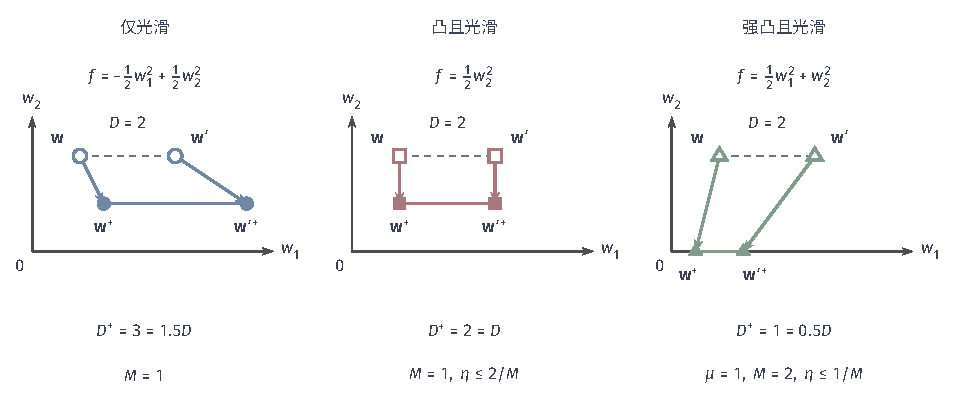
\includegraphics[width=161.957mm]{figures/03-foundations/02-learning-theory/tikz/learning-theory-curvature-stability/figure.pdf}
  \caption{同一梯度更新如何影响参数距离。三个参数平面使用相同尺度，初值均为
 $\bm w=(1,2)^\top$、$\bm w'=(3,2)^\top$，步长均为$\eta=1/2$。
 空心标记表示初值，实心标记表示$\bm w^+=\bm w-\eta\nabla f(\bm w)$及
 $\bm w'^{+}$；箭头表示各自的梯度步，虚线和实线连接更新前后的两点。
 图中二次函数的梯度步给出精确距离$D^+=3,2,1$，并非一般情形的距离等式。
 凸且$M$-光滑时，$\eta\leq2/M$保证不扩张；满足本章强凸光滑条件时，
 $\eta\leq1/M$保证至多以$1-\mu\eta$收缩。仅有光滑性不能排除扩张。}
 \label{fig:stability-curvature}
\end{figure*}
\FloatBarrier

因此，后面仍按上一节的两种算法分别分析。正则化路线修改经验目标：若加入足够强的二次项能使目标强凸，就可恢复最优解的稳定性，但必须检查惩罚是否造成不消失的偏差。SGD路线保留原目标：先计算扰动怎样沿迭代传播，再另外增加能够保证经验优化的条件。每条路线都要分别检查稳定性和经验优化，不能用其中一项的结论代替另一项。

\subsection{非凸学习问题的正则化}

对非凸损失，添加二次正则项要先补偿它的负曲率。以一维函数$-\kappa w^2/2$为例，加上$\lambda w^2/2$后得到$(\lambda-\kappa)w^2/2$；只有$\lambda>\kappa$时才强凸。一般地，若$\ell(\bm w,z)+\kappa\|\bm w\|_2^2/2$在凸决策集上为凸函数，就称损失为$\kappa$-弱凸，其中$\kappa\geq0$。在二阶可微的开凸域上，这等价于Hessian的所有特征值都不小于$-\kappa$。

上一小节的$(w^2-1)^2$就是一例：它的二阶导数为$12w^2-4\geq-4$，因而是4-弱凸的。加入$\lambda w^2/2$且$\lambda>4$后，导数为$w(4w^2-4+\lambda)$，括号内恒正，唯一的驻点也是最小点$w=0$。正则化确实把目标变成了强凸、解也变得稳定，可是这个解恰好是原损失为1的那个驻点，而原问题的最优损失为0。这个例子预示了下面定理中的代价项：为了消除负曲率所需的正则化强度，可能大到改变问题的答案。

若每条观测的损失都满足同一个弱凸上界$\kappa$，它们的平均也满足。加入强度$\lambda>\kappa$的二次正则项后，整个目标是$(\lambda-\kappa)$-强凸的；再保留Lipschitz条件，就可以复用凸正则化中比较两个最优解的证明。这里恢复的是修改后目标所确定的最优解的稳定性，并没有把原目标变成凸问题。
% 保留旧位置锚点，不再重复编号定义。
\phantomsection\label{def:weakly-convex}
\begin{theorem}[弱凸损失的正则化稳定性]
\label{thm:weakly-convex-regularization}
设$(Z,\mathcal Z)$为可测观测空间，
$\mathcal W=\{\bm w\in\mathbb R^d:\|\bm w\|_2\leq B\}$，其中$B\geq0$，
并设$\ell:\mathcal W\times Z\to\mathbb R$可测。固定$\kappa\geq0$和$L\geq0$；
对每个$z\in Z$，函数
$\bm w\mapsto\ell(\bm w,z)+\kappa\|\bm w\|_2^2/2$在$\mathcal W$上凸，且
\[
 |\ell(\bm u,z)-\ell(\bm v,z)|\leq L\|\bm u-\bm v\|_2
 \quad\text{对任意 }\bm u,\bm v\in\mathcal W.
\]
固定$n\geq1$并取$\lambda>\kappa$。对$S=(z_1,\ldots,z_n)\in Z^n$，假设
以下正则化目标的最小解存在，并定义可测算法
\[
 A_\lambda(S)=\argmin_{\bm w\in\mathcal W}
 \left\{\frac1n\sum_{i=1}^n\ell(\bm w,z_i)
 +\frac\lambda2\|\bm w\|_2^2\right\}.
\]
则对任意只相差一个观测的$S,S'\in Z^n$及任意$z\in Z$都有
\[
 |\ell(A_\lambda(S),z)-\ell(A_\lambda(S'),z)|
 \leq\beta_n,\qquad
 \beta_n\leq\frac{2L^2}{(\lambda-\kappa)n}.
\]
进一步固定$Z$上的概率分布$\mathcal P$，令$S\sim\mathcal P^n$，并令
$z\sim\mathcal P$独立于$S$。若独立测试损失、
训练损失以及每个固定$\bm w\in\mathcal W$的$\ell(\bm w,z)$均可积，则对任意固定
$\bm w\in\mathcal W$，定义
\[
 R_{\mathcal P}(\bm v)=\mathbb E_{z\sim\mathcal P}\ell(\bm v,z),
 \qquad
 \hat R_S(\bm v)=\frac1n\sum_{i=1}^n\ell(\bm v,z_i),
\]
并且
\[
 \mathbb E_S R_{\mathcal P}(A_\lambda(S))-R_{\mathcal P}(\bm w)
 \leq\frac{2L^2}{(\lambda-\kappa)n}+\frac\lambda2\|\bm w\|_2^2.
\]
\end{theorem}
\begin{proof}
正则化目标可以写成一个凸函数与
$(\lambda-\kappa)\|\bm w\|_2^2/2$之和，因而为$(\lambda-\kappa)$-强凸。
对相邻样本的两个最优解，重复定理~\ref{thm:regularized-erm-stability}的相加抵消论证，
即得稳定性界。由正则化目标的最优性，经验风险相对于固定比较参数的差不超过
$\lambda\|\bm w\|_2^2/2$。再加上期望泛化差就得到第二式。
\end{proof}

当$\kappa=0$时，这个界回到上一节的凸正则化结果。关键差别在$\kappa>0$时：为了使修改后的目标强凸，必须始终保持$\lambda>\kappa$，所以$\lambda$不能随样本量增加而趋于零；风险界中的正则化比较项因而不保证消失。稳定性项可以随$n$减小，仍不足以推出对原问题的PAC学习。这不是不可学习的结论，而是说明这条上界尚未完成学习证明。

定理假定算法求出正则目标的全局最小值。对这里确已强凸的正则目标，可行集上的局部最小值就是全局最小值；实际迭代若只返回近似解，还需控制求解误差。若正则项不足以抵消负曲率，则连强凸稳定性证明本身也不能使用。

\subsection{非凸学习问题的随机梯度下降}

另一条路线不修改原来的非凸目标，而是直接分析有限步SGD。沿用相邻样本、相同初值和共享索引序列的比较。与凸情形相比，每一步要计算两个来源：访问被替换观测时新加入的扰动，以及使用共同观测更新时对已有扰动的放大。下面先得到随步长和迭代次数变化的稳定性界；它只控制期望泛化差，尚未证明算法找到经验风险较小的解。

\begin{theorem}[非凸SGD的扰动传播]
\label{thm:nonconvex-sgd-product}
设$(Z,\mathcal Z)$为可测观测空间，
$\ell:\mathbb R^d\times Z\to\mathbb R$可测。对每个$z\in Z$，
$\ell(\cdot,z)$可微、$L$-Lipschitz且$M$-光滑，其中$M>0$，即
\[
\begin{aligned}
 |\ell(\bm u,z)-\ell(\bm v,z)|
 &\leq L\|\bm u-\bm v\|_2,\\
 \|\nabla\ell(\bm u,z)-\nabla\ell(\bm v,z)\|_2
 &\leq M\|\bm u-\bm v\|_2,
 \qquad \bm u,\bm v\in\mathbb R^d.
\end{aligned}
\]
固定$n,T\geq1$、确定初值$\bm w^{(0)}\in\mathbb R^d$及步长$\eta_t\geq0$。
给定$S=(z_1,\ldots,z_n)\in Z^n$，令算法内部随机数
$U=(i_0,\ldots,i_{T-1})$由独立且均匀分布于$\{1,\ldots,n\}$的索引组成；
当$S$随机时，$U$独立于$S$。算法更新
\[
 \bm w^{(t+1)}
 =\bm w^{(t)}-\eta_t\nabla\ell(\bm w^{(t)},z_{i_t}),
 \qquad t=0,\ldots,T-1.
\]
令$A_{n,T}(S,U)=\bm w^{(T)}$。比较相邻样本时，两次运行共享初值和$U$。
则任意只相差一个观测的$S,S'\in Z^n$及任意$z\in Z$都满足
\[
 \left|\mathbb E_U\ell(A_{n,T}(S,U),z)
 -\mathbb E_U\ell(A_{n,T}(S',U),z)\right|\leq\beta_{n,T},
\]
其中
\[
 \beta_{n,T}\leq\frac{2L^2}{n}
 \sum_{t=0}^{T-1}\eta_t\prod_{j=t+1}^{T-1}(1+M\eta_j).
\]
其中空乘积取1。若$\mathcal P$为$Z$上的概率分布，
$S\sim\mathcal P^n$，$U$独立于$S$，且独立测试损失与训练损失均可积，则
\[
 R_{\mathcal P}(\bm w)=\mathbb E_{z\sim\mathcal P}\ell(\bm w,z),
 \qquad
 \hat R_S(\bm w)=\frac1n\sum_{i=1}^n\ell(\bm w,z_i),
\]
并且
\[
 \left|\mathbb E_{S,U}
 [R_{\mathcal P}(A_{n,T}(S,U))-\hat R_S(A_{n,T}(S,U))]\right|
 \leq\frac{2L^2}{n}
 \sum_{t=0}^{T-1}\eta_t\prod_{j=t+1}^{T-1}(1+M\eta_j).
\]
\end{theorem}
\begin{proof}
在相邻样本上使用相同随机索引，记两次迭代参数的平均距离为$D_t$。
未抽中替换位置时，光滑性给出放大因子$1+M\eta_t$。
抽中时，在同一观测的更新之外，再加入两个观测的梯度差；梯度范数均不超过$L$，
所以新增距离至多$2L\eta_t$。由抽中概率$1/n$，
\[
 D_{t+1}\leq(1+M\eta_t)D_t+\frac{2L\eta_t}{n},\qquad D_0=0.
\]
逐步展开递推式，每一步产生的扰动都乘以后续更新的放大因子。
最后用Lipschitz性将$D_T$乘以$L$，即得损失差上界。
\end{proof}

步长固定为$\eta>0$时，把乘积按几何级数展开，得到
\[
 \beta_{n,T}\leq\frac{2L^2}{Mn}\bigl((1+M\eta)^T-1\bigr).
\]
与凸情形比较可以看出差距有多大。取$L=M=1$、$\eta=0.01$、$T=1000$（教学取值）：凸SGD的上界为$2\eta T/n=20/n$；这里$(1.01)^{1000}\approx2.1\times10^4$，上界约为$4.2\times10^4/n$，大了约两千倍。这个最坏情形上界允许指数放大，但并没有断言每个非凸算法的实际泛化差都指数增长。它说明的是：仅凭光滑性，无法为任意长的训练给出小的稳定性上界。减小步长、限制迭代轮数，或证明轨迹所在区域具有更好的曲率，都可以改善这个扰动估计。

还可以利用算法首次访问被替换位置的时间：在第一次抽中该位置之前，两条轨迹完全相同，没有任何差别。如果首次访问时步长已经减小，后续的放大效应就比从第一步开始估计时弱。下面给出Hardt、Recht与Singer这一思路的一个常数较宽松的版本\scite{hardt2016sgd}。

\begin{theorem}[递减步长的非凸SGD泛化界]
\label{thm:nonconvex-sgd-decay}
设$(Z,\mathcal Z)$为可测观测空间，
$\ell:\mathbb R^d\times Z\to[0,1]$可测。对每个$z\in Z$，
$\ell(\cdot,z)$可微、$L$-Lipschitz且$M$-光滑，其中$M>0$，即
\[
\begin{aligned}
 |\ell(\bm u,z)-\ell(\bm v,z)|
 &\leq L\|\bm u-\bm v\|_2,\\
 \|\nabla\ell(\bm u,z)-\nabla\ell(\bm v,z)\|_2
 &\leq M\|\bm u-\bm v\|_2,
 \qquad \bm u,\bm v\in\mathbb R^d.
\end{aligned}
\]
固定$n,T\geq1$、确定初值$\bm w^{(0)}\in\mathbb R^d$及$c>0$。
任取$Z$上的概率分布$\mathcal P$并令
$S=(z_1,\ldots,z_n)\sim\mathcal P^n$。算法内部随机数
$U=(i_0,\ldots,i_{T-1})$独立于$S$，并由独立且均匀分布于
$\{1,\ldots,n\}$的索引组成；算法以
$0\leq\eta_t\leq c/(t+1)$更新
\[
 \bm w^{(t+1)}
 =\bm w^{(t)}-\eta_t\nabla\ell(\bm w^{(t)},z_{i_t}),
 \qquad t=0,\ldots,T-1.
\]
令$A_{n,T}(S,U)=\bm w^{(T)}$，并在相邻样本上共享初值与$U$。定义$\beta_{n,T}$
为满足
\[
 \left|\mathbb E_U\ell(A_{n,T}(S,U),z)
 -\mathbb E_U\ell(A_{n,T}(S',U),z)\right|\leq\beta_{n,T}
\]
对任意只相差一个观测的$S,S'\in Z^n$及任意$z\in Z$成立的稳定性上界。
记$a=Mc$。对任意整数$1\leq t_0\leq T$，有
\[
 \beta_{n,T}\leq\frac{t_0}{n}
       +\frac{2L^2}{Mn}\left(\frac{T}{t_0}\right)^a.
\]
特别地，取$t_0=\lceil T^{a/(a+1)}\rceil$，可得
\[
 \beta_{n,T}\leq
 \frac{1+(1+2L^2/M)T^{a/(a+1)}}{n}.
\]
\end{theorem}
\begin{proof}
前$t_0$次抽样中至少一次选中替换位置的概率不超过$t_0/n$。
在这一事件上用损失差至多1估计。在其补事件上，两条轨迹在时刻$t_0$完全相同，
后续索引仍独立均匀，因而可从$D_{t_0}=0$开始使用前一定理的递推式。
利用$1+u\leq e^u$及调和和的积分上界，有
\[
 \prod_{j=t+1}^{T-1}\left(1+\frac a{j+1}\right)
 \leq\left(\frac T{t+1}\right)^a.
\]
所以后续的条件期望损失差至多为
\[
 \frac{2cL^2T^a}{n}\sum_{t=t_0}^{T-1}(t+1)^{-a-1}
 \leq\frac{2cL^2T^a}{an}\,t_0^{-a}.
\]
这里使用$\sum_{t=t_0}^{T-1}(t+1)^{-a-1}\leq\int_{t_0}^{T}x^{-a-1}\,dx\leq t_0^{-a}/a$。
合并两种事件，并代入$a=Mc$得到第一式。再代入所给$t_0$，利用
$T^{a/(a+1)}\leq t_0\leq T^{a/(a+1)}+1$即得第二式。
\end{proof}

第一式中的$t_0$是证明里人为选择的观察时刻，两项体现一种折中：$t_0$越大，前$t_0$步碰到替换位置的概率$t_0/n$越大；$t_0$越小，之后需要承受放大的步数越多，第二项越大。所给$t_0$使两项同阶。固定$L,M,c$并令$T=n$，这条递减步长稳定性上界为$n^{-1/(a+1)}$量级。更一般地，$T$按$n^p$增长且$p<(a+1)/a$时，上界仍趋于零。但到这里我们只知道训练风险与新数据风险在平均意义下相近；算法可能同时把两者维持在较高水平。要完成学习保证，还需要控制经验优化误差$\rho_{n,T}$，不能从稳定性界或驻点条件推断它已经很小。

为控制经验优化误差，需要把“梯度小”与“目标值接近最低值”联系起来。令$F$为固定样本的经验目标，$F_*=\inf_{\bm w\in\mathcal W}F(\bm w)$为有限实数。Polyak--\L{}ojasiewicz条件，简称PL条件，要求存在$\mu>0$，使
\[
 F(\bm w)-F_*\leq\frac{\|\nabla F(\bm w)\|_2^2}{2\mu}.
\]
于是，只要目标值仍明显高于$F_*$，梯度就不能接近零；梯度为零时必已达到最低目标值。这对梯度方法的意义在于：一步梯度下降使目标约下降$\eta\|\nabla F\|_2^2/2$，PL条件又保证这一下降量至少是当前误差$F-F_*$的$\mu\eta$倍，因此误差每步按比例缩小，呈几何衰减。凸性保证的是“没有坏的驻点”，PL条件用一个不等式直接保证了同样的效果，并且给出速率。它排除了本节开头那种高损失驻点，但不要求函数处处凸。这里控制的是目标值差，不是相邻样本上两个参数的距离，所以PL条件不能直接替代稳定性证明。

若PL不等式在整个指定区域内成立，称为区域PL条件。下面定理只要求它在每份样本的所有实际迭代点上成立，但常数$\mu$必须对这些样本和轨迹统一。观察到一次训练中的下降趋势，并不能验证这样的统一条件。
% 保留旧位置锚点，不再重复编号定义。
\phantomsection\label{def:pl-condition}

$F(w)=w^2/2$在$\mu=1$时PL不等式取等号；前面的$(w^2-1)^2$在$w=0$处违反条件，因为梯度为零而目标比最优值高1。非凸函数也可能满足PL，例如$w^2+3\sin^2w$在全局满足带正参数的PL条件，但它在部分位置的二阶导数为负\scite{karimi2016pl}。PL限制的是梯度与目标最优值差之间的关系，不是逐方向的曲率。

SGD使用的单样本梯度并不等于全量经验梯度。固定样本和当前参数后，随机抽取索引得到的梯度均值等于经验梯度，但还存在随机波动。下面用$\nu^2$限制这种梯度偏差的平均平方范数，用$D$限制初始经验优化误差，再用PL条件分析误差随迭代的下降。

为了同时得到风险界，下一个定理改为考察一次训练中保持不变的步长$\eta$，并使用前面的乘积型稳定性界，而不是直接拼接递减步长定理。证明中，光滑性估计一步更新后的目标值，PL条件把梯度范数换成经验优化误差，最后把优化误差与稳定性项相加。参数还必须始终留在这些条件成立的区域内。

\begin{theorem}[PL条件下非凸SGD的学习保证]
\label{thm:pl-stability-learning}
设$(Z,\mathcal Z)$为可测观测空间，
$\mathcal W\subseteq\mathbb R^d$为非空凸Borel区域，
并令$\mathcal O\subseteq\mathbb R^d$为包含$\mathcal W$的开集。
设$\ell:\mathcal O\times Z\to\mathbb R$可测，且各单样本损失在$\mathcal O$上
关于参数可微；存在$M>0$和$L\geq0$，使任意$\bm u,\bm v\in\mathcal W,z\in Z$都满足
\[
 \|\nabla\ell(\bm u,z)-\nabla\ell(\bm v,z)\|_2
 \leq M\|\bm u-\bm v\|_2,
 \qquad
 \|\nabla\ell(\bm u,z)\|_2\leq L.
\]
对每个允许分布$\mathcal P$，令$S=(z_1,\ldots,z_n)\sim\mathcal P^n$，
并定义
\[
 \hat R_S(\bm w)=\frac1n\sum_{i=1}^n\ell(\bm w,z_i),
 \qquad
 R_{\mathcal P}(\bm w)=\mathbb E_{z\sim\mathcal P}\ell(\bm w,z).
\]
固定初值$\bm w^{(0)}\in\mathcal W$、步长$0<\eta\leq1/M$及$T\geq1$。
令算法内部随机数$U=(i_0,\ldots,i_{T-1})$独立于$S$，其中各$i_t$独立且均匀
分布于$\{1,\ldots,n\}$，并更新
\[
 \bm w^{(t+1)}
 =\bm w^{(t)}-\eta\nabla\ell(\bm w^{(t)},z_{i_t}),
 \qquad t=0,\ldots,T-1.
\]
假定对所有样本和索引序列，全部迭代点均留在$\mathcal W$内。存在
$0<\mu\leq M$及$D\geq0$，使每个样本及其每个迭代点都满足
\[
\begin{aligned}
 \frac12\|\nabla\hat R_S(\bm w^{(t)})\|_2^2
 \geq\mu\!\left(
 \hat R_S(\bm w^{(t)})-\inf_{\bm w\in\mathcal W}\hat R_S(\bm w)\right),\\
 \hat R_S(\bm w^{(0)})-\inf_{\bm w\in\mathcal W}\hat R_S(\bm w)\leq D.
\end{aligned}
\]
进一步设存在$\nu\geq0$，使对所有$S\in Z^n$和$\bm w\in\mathcal W$都有
\[
 \frac1n\sum_{i=1}^n
 \|\nabla\ell(\bm w,z_i)-\nabla\hat R_S(\bm w)\|_2^2\leq\nu^2.
\]
假定独立测试损失$\ell(\bm w^{(T)},z)$、训练损失
$\ell(\bm w^{(T)},z_i)$及每个固定$\bm w\in\mathcal W$的$\ell(\bm w,z)$均可积，
并且经验风险与期望风险的下确界为有限实数且可测。则
\begin{align*}
 &\mathbb E_{S,U}R_{\mathcal P}(\bm w^{(T)})-
   \inf_{\bm w\in\mathcal W}R_{\mathcal P}(\bm w)\\
 &\quad\leq\frac{2L^2}{Mn}\bigl((1+M\eta)^T-1\bigr)
                  +D(1-\mu\eta)^T+\frac{M\eta\nu^2}{2\mu}.
\end{align*}
\end{theorem}
\begin{proof}
定理~\ref{thm:nonconvex-sgd-product}的轨迹比较给出第一项均匀稳定性上界。
为分析经验优化误差，固定样本及此前的迭代结果，记
$\bm g_t=\nabla\ell(\bm w^{(t)},z_{i_t})$。
条件均值满足$\mathbb E\bm g_t=\nabla\hat R_S(\bm w^{(t)})$，条件二阶矩满足
\[
 \mathbb E\|\bm g_t\|_2^2
 \leq\|\nabla\hat R_S(\bm w^{(t)})\|_2^2+\nu^2.
\]
将更新代入光滑性不等式，并对当前索引取期望，得到
\begin{align*}
 \mathbb E\hat R_S(\bm w^{(t+1)})
 &\leq\hat R_S(\bm w^{(t)})
 -\frac\eta2\|\nabla\hat R_S(\bm w^{(t)})\|_2^2
 +\frac{M\eta^2\nu^2}{2}.
\end{align*}
这里用$\eta\leq1/M$，将光滑性展开中梯度范数平方的系数控制为$-\eta/2$。再用PL条件，把这一负项换成当前经验目标差的$-\mu\eta$倍。减去固定样本的最低经验风险，再对此前的索引平均，记得到的经验优化误差为$e_t$，便有
\[
 e_{t+1}\leq(1-\mu\eta)e_t+\frac{M\eta^2\nu^2}{2},
 \qquad e_0\leq D.
\]
求和几何级数，得到
$e_T\leq D(1-\mu\eta)^T+M\eta\nu^2/(2\mu)$。
这个上界对每份样本都成立。再对样本取平均，并加上前面得到的期望泛化差上界，由定理~\ref{thm:generalization-optimization-learning}得到所述超额期望风险界。
\end{proof}

这三项分别来自两个证明。第一项来自相邻样本轨迹的稳定性，估计期望泛化差；第二项$D(1-\mu\eta)^T$和第三项$M\eta\nu^2/(2\mu)$一起估计经验优化误差。增加$T$使第二项下降，却可能增大第一项；固定非零步长且$\nu>0$时，第三项不会随$T$下降。若使用全梯度，$\nu=0$，但仍要为实际的全梯度更新建立相应稳定性界，不能只从公式中删除方差项就省去算法核验。

要使三项同时趋于零，可以随样本量调整整次训练的步长和时长。要求$L,M,D,\nu$有不依赖分布和样本量的上界，且PL常数$\mu$有统一的正下界。取$\eta_n=n^{-r}$（$r>0$），在每次训练内部保持这个步长不变，并令$T_n=\lfloor c_0\log n/\eta_n\rfloor$，其中$0<c_0<1/M$。此时总步长约为$c_0\log n$：足以让初始优化误差衰减，又不至于使扰动放大项超过样本量带来的改善。三个上界分别为$O(n^{Mc_0-1})$、$O(n^{-\mu c_0})$和$O(n^{-r})$，都趋于零。因此在这些统一条件下可以得到PAC学习保证。

这也回答了本节的问题：非凸性并不自动排除学习，但只证明算法稳定或梯度变小都不够。正则化路线还要控制改动目标的代价，SGD路线还要控制经验优化误差；任何一项没有得到保证，都不能把已有的泛化界称为完整的学习结论。

\section{本章小结}
\label{sec:general-learning-summary}

本章把一般学习的风险保证分为两部分：用样本评价输出时有多大偏差，算法的经验风险离训练样本上的最低值还有多远。一致收敛同时估计比较决策空间中全部决策的风险，稳定性则直接分析算法的输出，二者都要结合经验优化。对有界损失类，在允许全部分布且满足本章可测性条件时，各正尺度的胖打散维有限刻画一致收敛；有限伪维是更强的充分条件。一般学习可能不满足一致收敛，仍可由合适的算法完成。

在有界损失、恰当输出、允许全部观测分布及所列可测性条件下，一般学习基本定理把可学习性刻画为算法的存在性：存在一个对内部随机性平均后均匀稳定、且对每份样本都渐近经验最优的算法。证明允许重新构造算法，并不要求原来的每个学习算法都稳定。经验最优性排除了“稳定但始终选择高风险决策”的情况；稳定性也不能脱离经验最优性单独作为学习目标。

各类稳定性的保证取决于各自的比较方式。留一法联系$n$项与$n-1$项算法；平均替换直接对应期望泛化差；均匀替换在有界损失下还能支持高概率的集中不等式。参数距离要先经Lipschitz性或非负光滑损失的自界关系转换为损失差；互信息和条件互信息则通过参照分布把统计依赖转化为风险代价。无论走哪条路线，由平均风险得到允许族上的统一PAC保证时，经验优化误差都必须趋于零，而且两项速率必须对该族内所有分布统一；允许全部相关分布时，才称为分布无关PAC保证。

具体算法的证明都需要把这两部分接起来，这也是开篇所说各项条件的用途。Lipschitz性把参数距离换算成损失差，弥补了零一损失随参数跳变的缺陷；光滑性控制一次梯度更新对两条轨迹距离的影响；凸性使经验优化误差可以随迭代算出，并配合光滑性保证同一观测的更新不扩大距离。正则化与稳定性的联系落在强凸性上：正则项使目标在最优解附近按距离平方增长，相邻样本的最优解因而至多相距$2L/(\lambda n)$；代价是目标偏离原经验风险，$\lambda$需在两者之间折中。凸SGD则先比较相邻样本的轨迹，再用凸性分析平均输出的经验风险。非凸正则化即使恢复了稳定性，惩罚代价也未必消失；非凸SGD则需要分别处理扰动放大和经验优化，PL条件只解决后一个问题。下一章将继续用这些区分分析神经网络，而不是只依据训练损失下降判断能否泛化。

\paragraph{扩展阅读}
Shalev-Shwartz等人的论文在一般损失框架中比较了可学习性、稳定性与一致收敛。阅读时可结合本章的基本定理，检查各渐近经验最优条件平均了哪些随机量，以及必要性证明为什么允许重新构造算法\scite{shalevshwartz2010learnability}。

Bousquet与Elisseeff讨论了稳定性如何进入风险与集中不等式；Hardt、Recht与Singer进一步分析了SGD。对照阅读时，可以追踪同一条观测的梯度更新是否收缩、替换观测怎样引入扰动，以及这些递推在凸与非凸情形下有何不同\scite{bousquetelisseeff2002,hardt2016sgd}。

Steinke与Zakynthinou的条件互信息分析把学习、样本压缩和信息量联系起来。阅读时可回到本章的双样本构造，分别写出真实的联合分布与“重新抽取选择变量”的参照分布，看清它与普通互信息的参照过程为何不同\scite{steinke2020conditional}。
